\documentclass[]{article}
\usepackage{amsmath}
\usepackage{amssymb}
\usepackage{color}
\usepackage{fancybox}
\usepackage{graphicx}
\usepackage[pdftex,colorlinks]{hyperref}
\usepackage{pdfpages}
\renewcommand*\rmdefault{cmdh}
%\usepackage[T1]{fontenc}
\newcommand{\superscript}[1]{\ensuremath{^{\textrm{#1}}}}
\newcommand{\subscript}[1]{\ensuremath{_{\textrm{#1}}}}
\renewcommand{\thesection}{}

\def\thesection{\arabic{section}}
\def\thesubsection{\arabic{section}.\arabic{subsection}}
\def\thesubsubsection{\arabic{section}.\arabic{subsection}.\arabic{subsubsection}}

\begin{document}
\rmfamily
\setcounter{secnumdepth}{3}

	% Cover Page
	\begin{titlepage}
		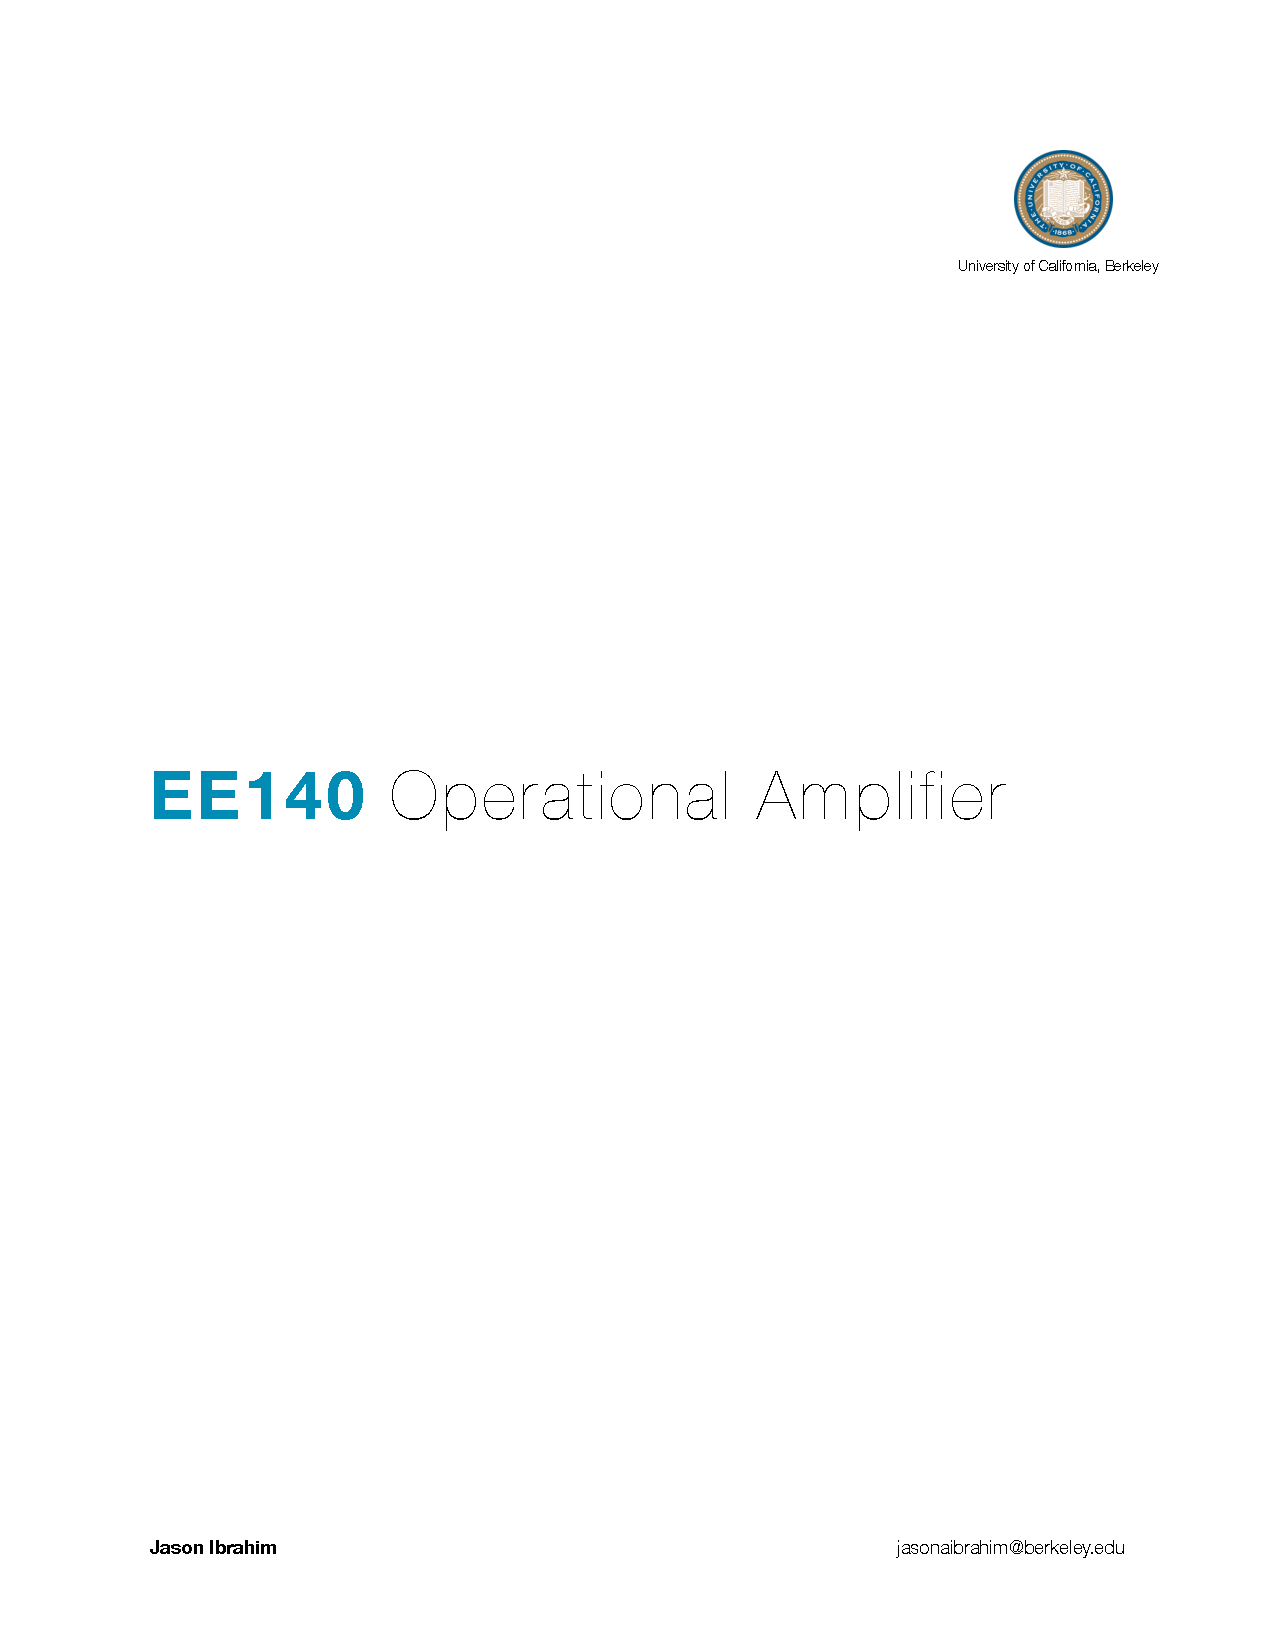
\includepdf[pages={1}]{title_page.pdf}	
	\end{titlepage}
	
	% Introduction
	
	\section{Introduction}
		As the demand for mixed mode integrated circuits increases, the design of analog circuits such as operational amplifiers in CMOS technology becomes more critical. This technology has become an integral part of many integrated circuit chips fabricated today in a number of application areas. These amplifiers offer a number of advantages in terms of power dissipation, die area, and compatibility with digital circuits when compared to their bipolar counterparts.
	
		In this paper we design and simulate a specific, widely used operational amplifier architecture, showing in detail how the formulation of the design variables takes place through a number of equations derived and calculated by hand. We then simulate the amplifier using HSPICE, presenting performance measures such as unity-gain bandwidth, open-loop gain, and settling time. We show how the proposed amplifier meets the specifications set in place by the project guidelines. We conclude with a discussion of the characteristics of the amplifier and the overall experience of the design project.
		
		% Circuit Schematic
		\begin{figure}
			\subsection{Circuit Schematic}
			\includegraphics[width=1.2\textwidth]{CMOS_complete.pdf}
			\caption{Two stage op-amp considered in this paper.}
		\end{figure}
		\newpage
	
	% Hand Analysis Begins Here...
	\section{Part I: Hand Analysis}
		For the purposes of designing this amplifier, the design approach is as follows. First, we lay the groundwork for all important equations that must be considered in order to meet the specifications. We note dependencies and realize variables that enable design control. We then begin with the most rigorous specifications and choose our variables to be within margins that exceed the requirements, to provide a safety cushion against non-idealities. We keep all constraints in mind and finalize a design. We confirm that the requirements are met.
	
		\subsection{Equations}
	
		In this section, all of the relevant equations required to meet the specifications are listed for the purposes of demonstrating the interdependencies between variables and to illustrate the design process of the amplifier.
		$$$$
		Specifications to be met:
	
		\begin{itemize}
			\item Gain $\ge 1500 $
			\item Output Swing : 1.2V
			\item Settling Time : 8ns with 0.4V step
			\item Unity Gain Frequency $\ge 600 MHz$
			\item Common Mode Input Range: 0.8V
			\item CMRR $\ge 75dB$
			\item PSRR $\ge 60dB |_{DC} \ \ 50dB$ at 1MHz
			\item Power Dissipation: 1.5mW
		\end{itemize}
	
		\pagebreak 
	
			\subsubsection{Settling Time}
				$$$$
				To meet this specification, we will design our amplifier to have a slew rate that is one tenth of the settling time. Although this is not a one to one correspondence with the specification, settling time and slew rate are closely related, and achieving the above margin is a good indication that the spec has been met.\footnote{\tiny C. T. Nguyen, Lecture 24, April 25, 2013}


				$$ SR = \frac{10V_{0}}{T_{s|0.1\%}}$$
				$$T_{s|0.1\%} = 8ns \ \ with\ \  0.4V Step$$
				$$ SR = \frac{10(0.4)}{8ns}$$
				$$SR = 500 \frac{V}{\mu S} $$
				$$SR = \frac{I_{xm}}{C} $$

				\begin{center}\framebox{$\frac{I_{xm}}{C_{}} \ge 5\times10^{8} V/s $}\end{center}
				where C is the largest capacitance in the circuit, and Ixm is the limiting current.
				$$$$
		
			\subsubsection{Unity Gain Frequency}
				$$$$
				$$ugf= \frac{gm_{I}}{C_{}} $$
				$$ugf = 2\pi 600MHz$$
				\begin{center}\framebox{$\frac{gm_{I}}{C_{}} \ge 2\pi 600 MHz $}\end{center}
		

			\subsubsection{Phase Margin}
				$$$$
				Phase margin, settling time, and unity gain frequency are all closely related and impact the stability of the circuit in feedback. Aiming for a target phase margin that is conducive to meeting the above two specs,
				$$PM = 65^{\circ}$$
				$$\omega_{p2} \ge tan(65)\times 2\pi 600Mhz$$
				\begin{center}\framebox{$\frac{gm_{II}}{C_{I}+C_{II}} \ge tan(65)\times 2\pi 600MHz$}\end{center}
				\pagebreak
		
			\subsubsection{Gain}
				$$$$
				Total Gain: $A_{v} = A_{v_{1}}A_{v_{2}}$

				$$ A_{v_{1}} = gm_{3}\left(\frac{\frac{V_{A4}}{I_{D3}}\frac{V_{A5}}{I_{D3}}}{\frac{V_{A4}}{I_{D3}}+\frac{V_{A5}}{I_{D3}}}\right) \ \ \ \ \ \ \ \ \ \ A_{v_{2}} = -gm_{6}\left(\frac{\frac{V_{A6}}{I_{D6}}\frac{V_{A9}}{I_{D6}}}{\frac{V_{A6}}{I_{D6}}+\frac{V_{A9}}{I_{D6}}}\right)$$
				\newline
				$$ A_{v} = \frac{-gm_{3}gm_{6}}{I_{D3}I_{D6}}\left(\frac{V_{A4}V_{A5}}{V_{A4}+V_{A5}}\right)\left(\frac{V_{A6}V_{A9}}{V_{A6}+V_{A9}}\right) \footnote{\tiny Paul Gray, Robert Meyer, "Analysis and Design of Analog Integrated Circuits" (Wiley and Sons, 2010), 423}$$
				\newline
				Using the relation $ \frac{gm}{I_{D}} = \frac{2}{r_{0}} $ gives us
				\newline
				$$ A_{v} = \frac{-4}{V_{ov3}V_{ov6}}\left(\frac{\frac{1}{\lambda_{n}}\frac{1}{\lambda_{p}}}{\frac{1}{\lambda_{n}}+\frac{1}{\lambda_{p}}}\right)^2$$
				$$A_{v}= \frac{32.65}{V_{ov3}V_{ov6}}$$
				\begin{center}\framebox{$\frac{32.65}{V_{ov3}V_{ov6}} \ge 1500$}\end{center}
		
			\subsubsection{Output Swing}
				$$$$
				In order to satisfy an output swing of 1.2V we must satisfy the following:
				$$ V_{out, _{max}}  = V_{DD} - V_{ov_{9}} = 1.35 V $$
				$$ V_{out, _{min}}  =  V_{ov_{6}} = 0.15 V$$
				\begin{center}\framebox{$V_{ov9} \le 0.15V$}\end{center}
				\begin{center}\framebox{$V_{ov6} \le 0.15V$}\end{center}
				\pagebreak
		
			\subsubsection{Common Mode Rejection Ratio}
				$$$$
				\begin{center}
				CMRR = $|\frac{A_{dm}}{A{cm}}|$
				\end{center}
		
				The common mode rejection ratio is only dependent upon the first stage of the amplifier, because the second stage is a single ended input and output.
				\newline
				\begin{center}
				CMRR = $2gm_{3}r_{07}gm_{2}(r_{03} || r_{02})$

				= $\frac{4}{V_{ov3}V_{ov2}}\left(\frac{\frac{1}{\lambda_{n}}\frac{1}{\lambda_{p}}}{\frac{1}{\lambda_{n}}+\frac{1}{\lambda_{p}}}\right) \footnote{\tiny Paul Gray, Robert Meyer, "Analysis and Design of Analog Integrated Circuits" (Wiley and Sons, 2010), 427} $

				\end{center}
				\begin{center}\framebox{$\frac{11.43}{V_{ov3}V_{ov2}} \ge 75dB$}\end{center}
		
			\subsubsection{Power Supply Rejection Ratio}
		
				In calculating the PSRR, we will neglect the variations due to the positive supply, $V_{DD}$. This is because $PSRR_{+}\rightarrow \infty $ for low frequencies with perfect matching \footnote{\tiny Paul Gray, Robert Meyer, "Analysis and Design of Analog Integrated Circuits" (Wiley and Sons, 2010), 431}. This analysis is shown in G$\&$M page 431.

				Instead, we will calculate the PSRR that emerges due to variations from the $V_{SS}$ supply, which in this case is ground.
				$$A_{-} = \frac{v_{o}}{vss} = \frac{r_{09}}{r_{06}+r_{09}} = \frac{\frac{1}{\lambda_{p}}}{\frac{1}{\lambda_{n}}+\frac{1}{\lambda_{p}}} \footnote{\tiny Paul Gray, Robert Meyer, "Analysis and Design of Analog Integrated Circuits" (Wiley and Sons, 2010), 431}$$
				$$PSRR = \frac{A_{dm}}{A_{-}}$$
				\begin{center}\framebox{$\frac{A_{dm}}{0.5714} \ge 60 dB$}\end{center}
			
				\pagebreak
		
			\subsubsection{Common Mode Input Range}
		
				When $V_{IC}$ is reduced to the point where $ V_{GD_{3}} = V_{GD_{5}}  = V_{t_{3}} = V_{t_{5}}, M3 $ and $ M5 $ operate at the edge of saturation. 
				Thus, we define the lower end of the common mode input range to be :

				$$ V_{IC} \ge V_{t_{3}} + V_{t_{2}}+V_{ov_{2}}  $$
				$$ V_{IC} \ge V_{ov_{2}}  $$

				The specification calls for a common mode input range that is $ 0.8V $ inside the output swing range. This gives us a constraint on $  V_{ov_{2}} $

				$$ V_{IC_{min}} = 0.125 V $$
				\begin{center}\framebox{$ V_{ov_{2}}  \le 0.125V$}\end{center}

				If $ V_{IC} $ is too high, we have $M7$ falling into the triode region. Examining the drain voltage of $ M7,$

				$$ V_{DS_{7}} = V_{IC} - V_{GS_{3}} -V_{DD} = V_{IC} - V_{t3} - V_{ov_{3}} - V_{DD} $$

				Therefore, $ V_{IC} $ must satisfy the following:

				$$ V_{IC} < V_{DD_{}}  -	| V_{t_{3}}| - |V_{ov_{3}}| - |V_{ov_{7}}| $$
				$$ V_{IC} < 1.5  -0.3 - |V_{ov_{3}}| - 0.15 $$
				$$ V_{IC} < 1.05 - |V_{ov_{3}}|  $$
				From the specification,
				$$V_{IC_{max}} = 0.925 V$$
				$$ 0.925 < 1.05 - |V_{ov_{3}}|  $$
				\begin{center}\framebox{$ |V_{ov_{3}}| < 0.125$}\end{center}
	
				\pagebreak
				
		\subsection{Design Equations and Sizing}
			In this section, we illustrate the design process of the amplifier. With the knowledge of the equations and constraints, we are able to make design decisions. These design decisions are based partly on intelligent speculations and in a large part on the equations and constraints. We complete the design with dimensions for each transistor and the value of the compensating capacitor, $C_{c}$.
			$$$$
			For consistency with the load capacitance, we choose $C_{c}$ to be 2pF. This gives us the following:
			\subsubsection{Slew Rate}
				$$\frac{I_{xm}}{2pF} \ge 500 000 000 $$
				$$I_{xm} \ge 1mA$$
		
			\subsubsection{Unity Gain Frequency}
				$$\frac{gm_{I}}{2pF} \ge 2\pi 600 MHz $$
				$$gm_{I} \ge 7.53mS$$
		
			\subsubsection{Output Swing}
			$$V_{ov9} \le 0.15V$$
			$$V_{ov6} \le 0.15V$$

			To have a comfortable margin, we set $V_{ov6,9} = 0.09 V$	
		
			\subsubsection{Gain}
				$$\frac{32.65}{V_{ov3}V_{ov6}} \ge 1500$$
				With $V_{ov6} = 0.09$,
				$$v_{ov3} \le 0.24 V $$
				Set $V_{ov3} = 0.1V$ to satisfy the common mode input range spec.
				$$$$

				\pagebreak
		
			\subsubsection{Sizing of M3, M5}
				To reduce capacitances and minimize power and current consumption, set all channel lengths to the minimum value, $L_{min} = 130 nm$.
				$$ gm_{3} = k_{p}'W/L(V_{ov}) $$
				$$ 0.00753 = k_{p}'W/L(0.1) $$
				$$ W/L_{3,5} = 73712/130 $$
			
			\subsubsection{Sizing of M7, M9}
				$$$$
				As we can see from the settling time constraint, the circuit requires the maximum current we have available given the power restriction. With this in mind, we choose a reasonable value from experience and set the current through M9 to be 375 microamps and bias the output at half of the supply voltage. In addition, we match transistors 7 and 9 to ensure that the settling time specification is met, since both transistors supply current through large capacitors.
				$$0.5k_{p}'(W/L)_{}(V_{ov})^2(1+0.15(V_{SD}) = 375 \mu A $$
				$$0.5k_{p}'(W/L)_{}(0.09)^2(1+0.15(0.75) = 375 \mu A $$
				$$W/L_{7,9} = 81474/130$$
			
			\subsubsection{Sizing of M1}
				$$$$
				In order to meet the power dissipation requirement, the current through M1 must be no more than 250 microamps.
				$$0.5k_{p}'(W/L)_{}(V_{ov})^2(1+0.15(V_{ov}+V_{t}) = 250 \mu A $$
				$$0.5k_{p}'(W/L)_{}(0.09)^2(1+0.15(0.39) = 250 \mu A $$
				$$W/L_{1} = 57087/130$$
			
			\subsubsection{Sizing of M6}
				$$0.5k_{n}'(W/L)_{}(V_{ov})^2(1+0.2(0.75) = 375 \mu A $$
				$$0.5k_{n}'(W/L)_{}(0.09)^2(1+0.2(0.75) = 375 \mu A $$
				$$ W/L_{6} = 31527/130 $$
			
			\subsubsection{Sizing of M2, M4}
				$$$$
				From common mode input range,
				$$V_{ov2,4} \le 0.15V $$
				At equality we have,
				$$0.5k_{n}'(W/L)_{}(V_{ov})^2(1+0.2(V_{DS}) = 188 \mu A $$
				The drain-source voltage of M4 is the Vgs of M6. With this in mind,
				$$0.5k_{n}'(W/L)_{}(0.15)^2(1+0.2(0.39) = 188 \mu A $$
				$$W/L_{2,4} = 6053/130 $$
			
			\subsubsection{RHP Zero}
				$$$$
				We want to set the resistor, $R_{z}$, to a value such that the zero introduced by the circuit is pushed out to infinity. To do this we set,
				$$ R_{z} = 1/gm_{II} $$
				$$ gm_{II} = k_{n}'W/L(V_{ov}) = 7.24 mS $$
				$$R_{z} = 138 \Omega$$
				$$R_{z} = L/(Wk_{n}'(V_{GS}-V_{t})) $$
				$$ W/L_{r} = 2012/130 $$
			
			\subsubsection{Frequency Response}
				$$$$
				We would like to impart a phase margin of 60 degrees or better to offer a circuit that is stable under unity gain feedback and yields a quick settling time for sharp rising signals. To this end, we must push the second pole out past the value shown in the equations section above. In order to satisfy this, we must meet the following constraint,
				$$C_{I}+C_{II} \le 8.96\times 10^{-13}$$
				The calculations involving the derivation of the capacitances is shown in a\\ MATLAB script below and we can see that the requirement is met. We have included the estimated areas and relevant perimeters of the drain and source of the transistors as per the project guidelines.
		
				\pagebreak
				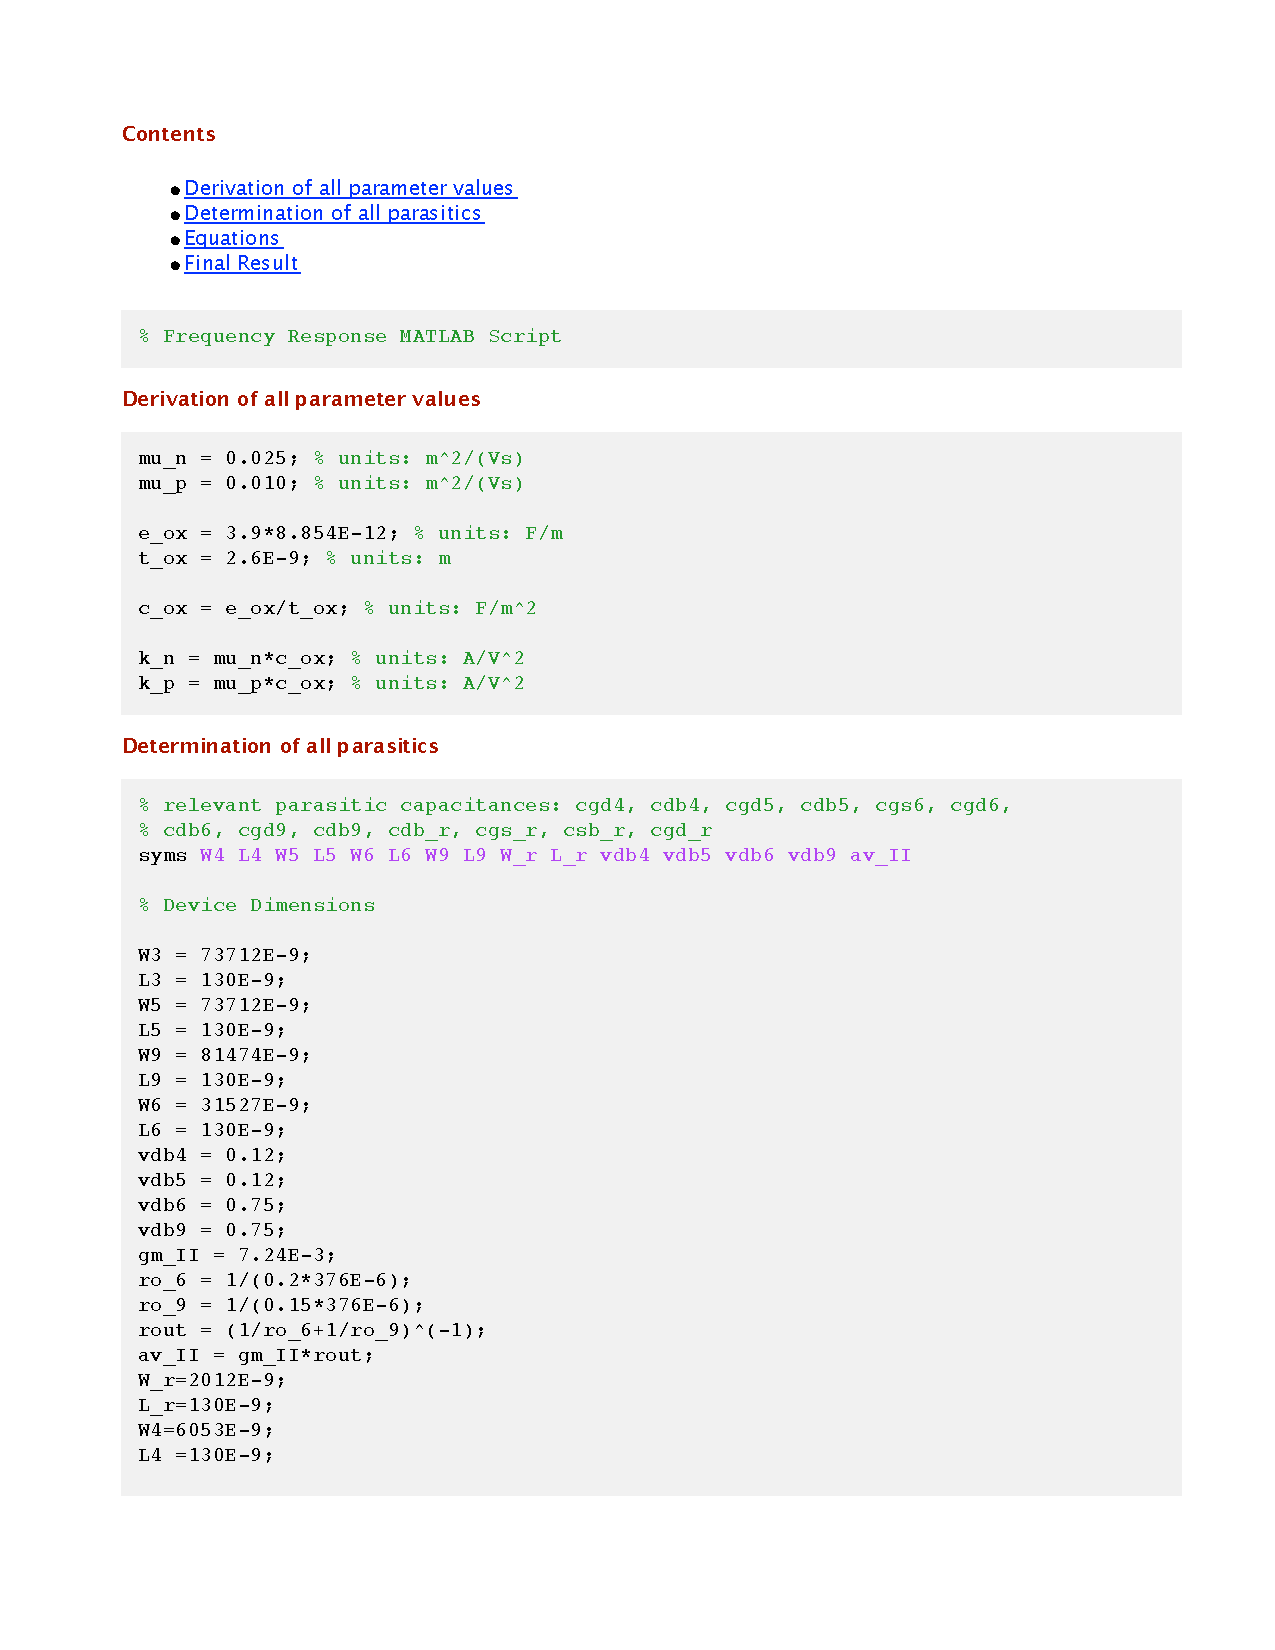
\includepdf[pages={1}]{matlab_script.pdf}
				\includepdf[pages={2}]{matlab_script.pdf}	
		
	\section{Part II: Simulation}
		We go from the design parameters we have just derived and simulate the op-amp in hspice. We make adjustments to certain dimensions as necessary for biasing. For instance, the width of M6 had to be reduced in order to allow for saturation conditions for all transistors. Other transistors were adjusted to reduce power consumption. We make adjustments to certain dimensions as necessary for the fulfillment of specifications as well. Slight tweaking of all transistors is required in order to comply with the 65nm technology used for this design. Transistors were also sized to reduce or increase overdrive voltages. Through many iterations, the devices are sized in such a way that the project parameters are all met. Dimensions used in the simulation of the circuit are within 10 percent of the estimated values except where noted. Wherever variances lie, the hand calculated values rectify these disparities when the values in the equations used in the above calculations are substituted with values from the simulation.\\ \\
		We have met all of the specifications called for in the design and have done so adequately. Graphs, tables and simulated values are now shown to substantiate the performance of this op-amp.
		

		\begin{figure}
			\subsection{Transistor and Bias Summary}
				$$$$
				\subsubsection{Biasing and small signal parameters}
				As we can see, all bias currents are within $10\%$ of hand calculated values. The overdrive voltage of $M1,7,9$ were further reduced to increase efficiency.
				
				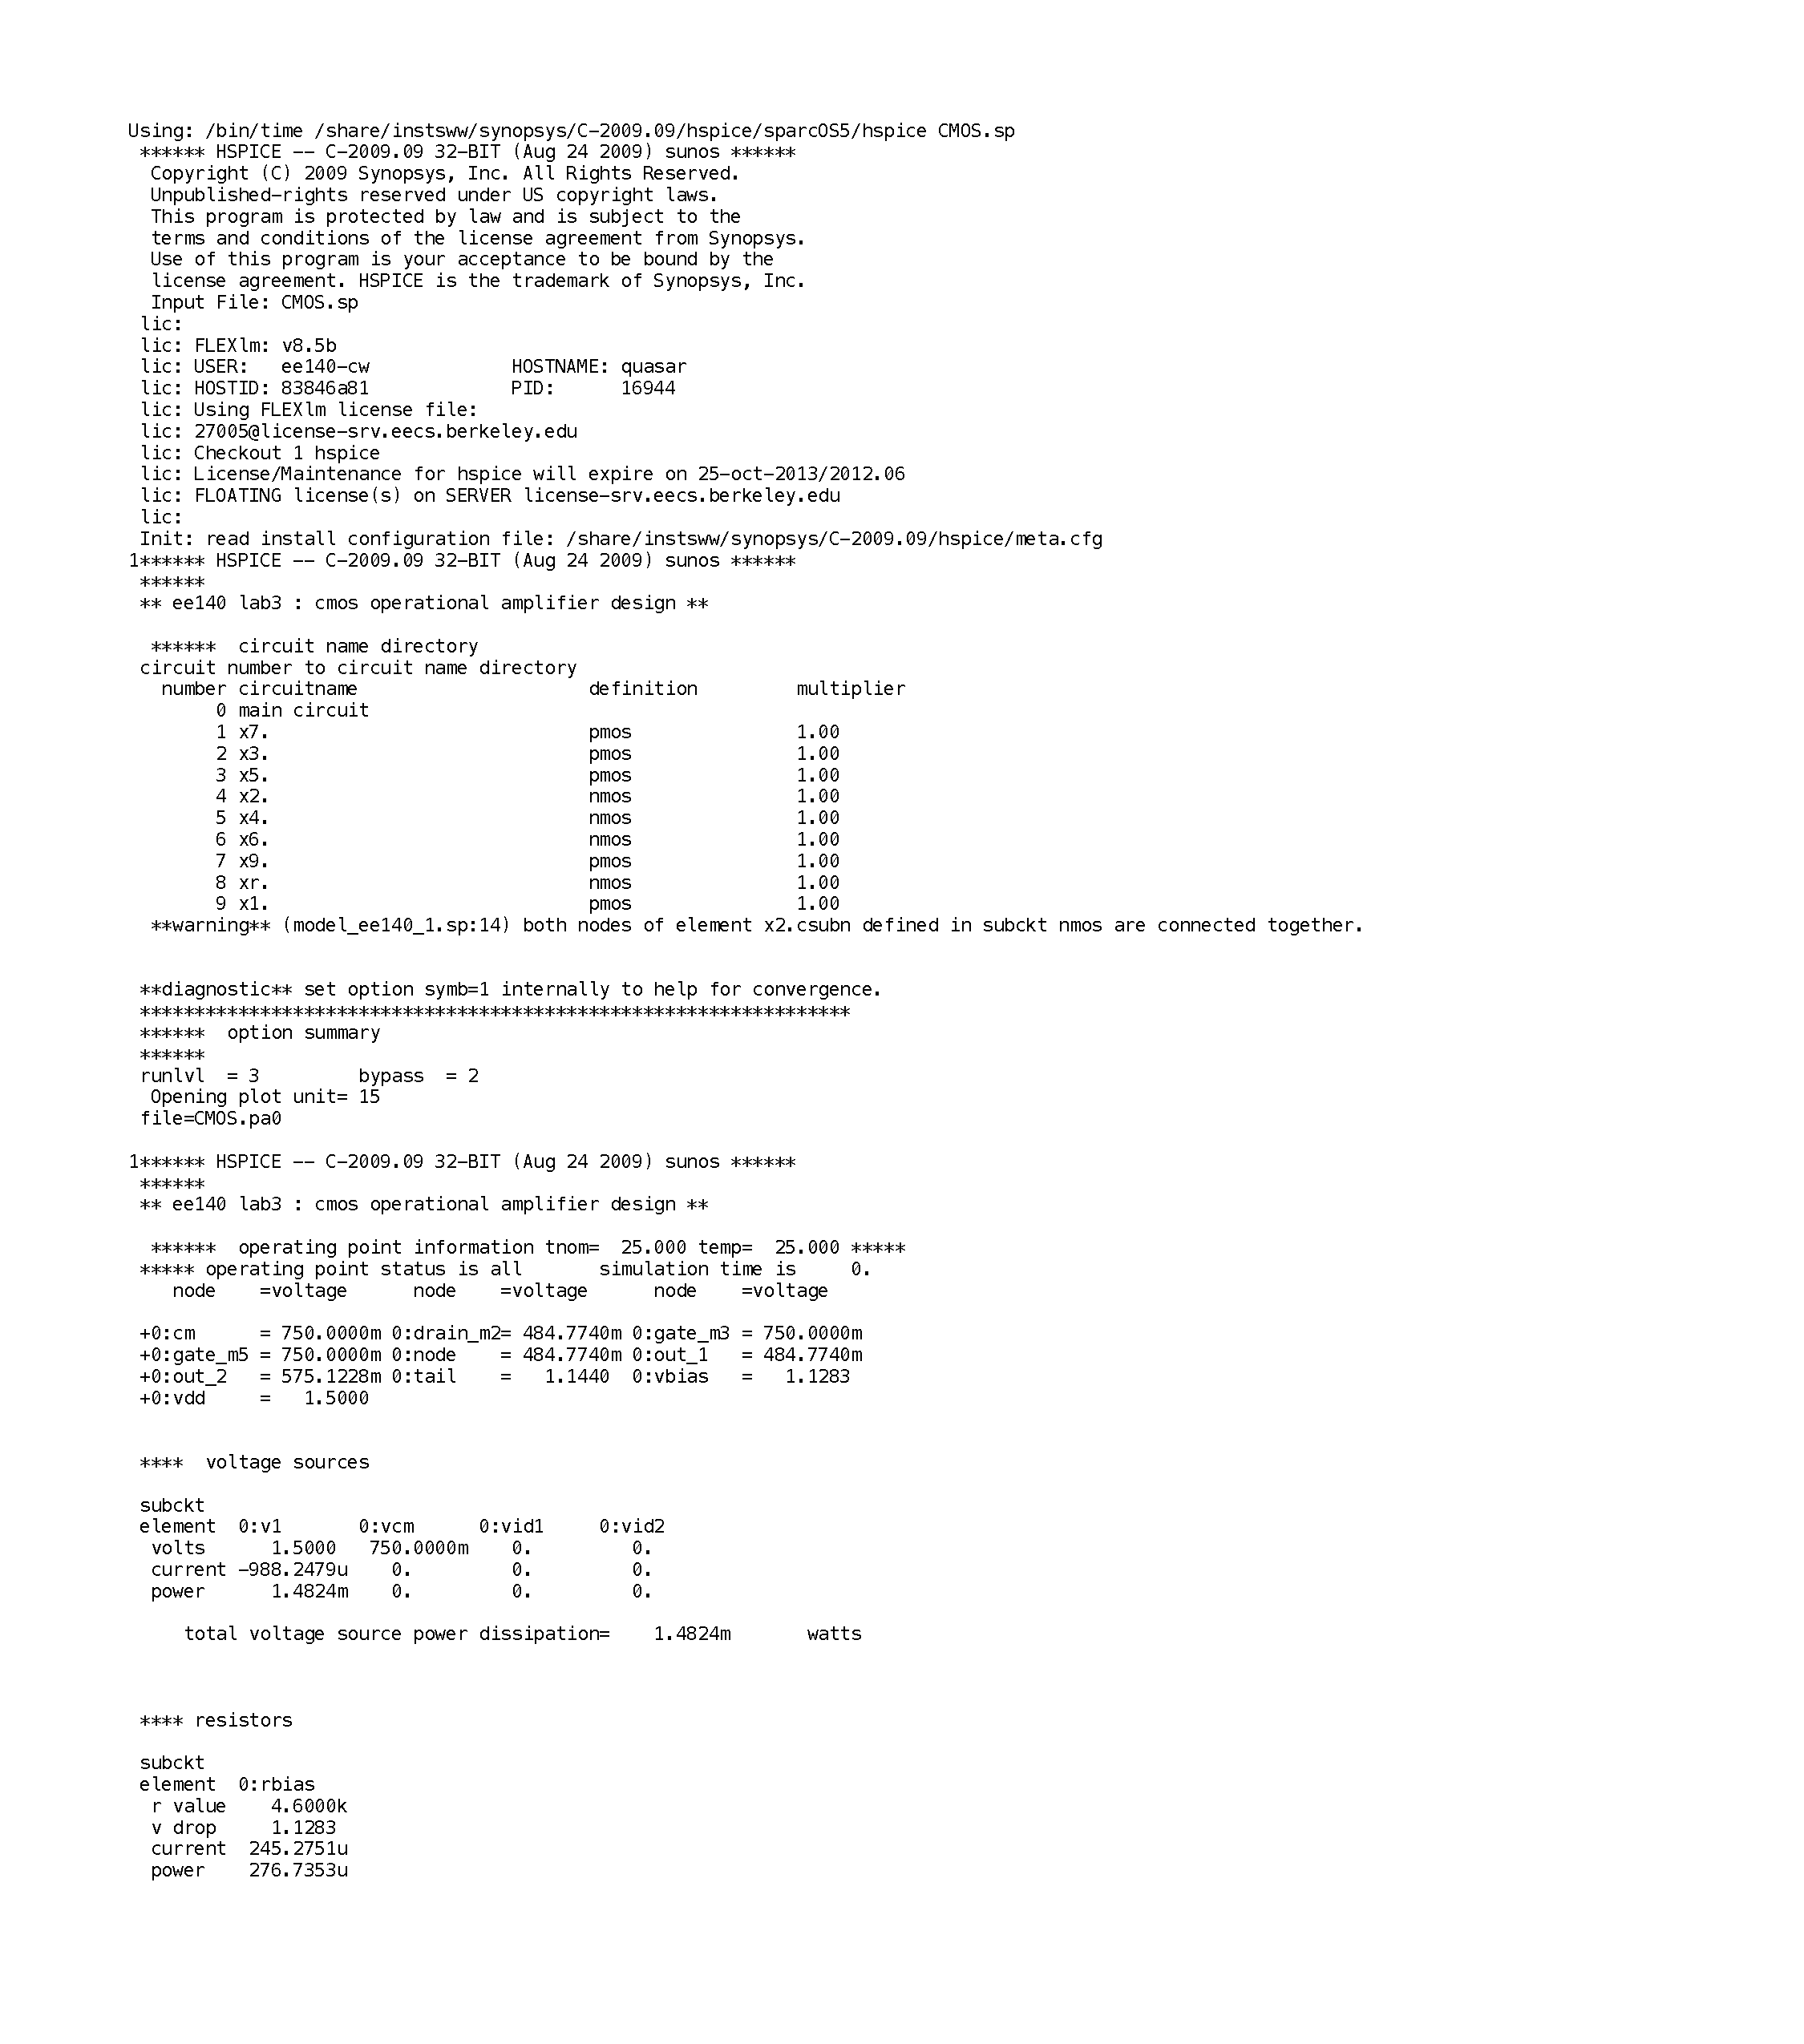
\includegraphics[width=1.25\textwidth]{operating_point.pdf}
		\end{figure}
		
		\begin{figure}
			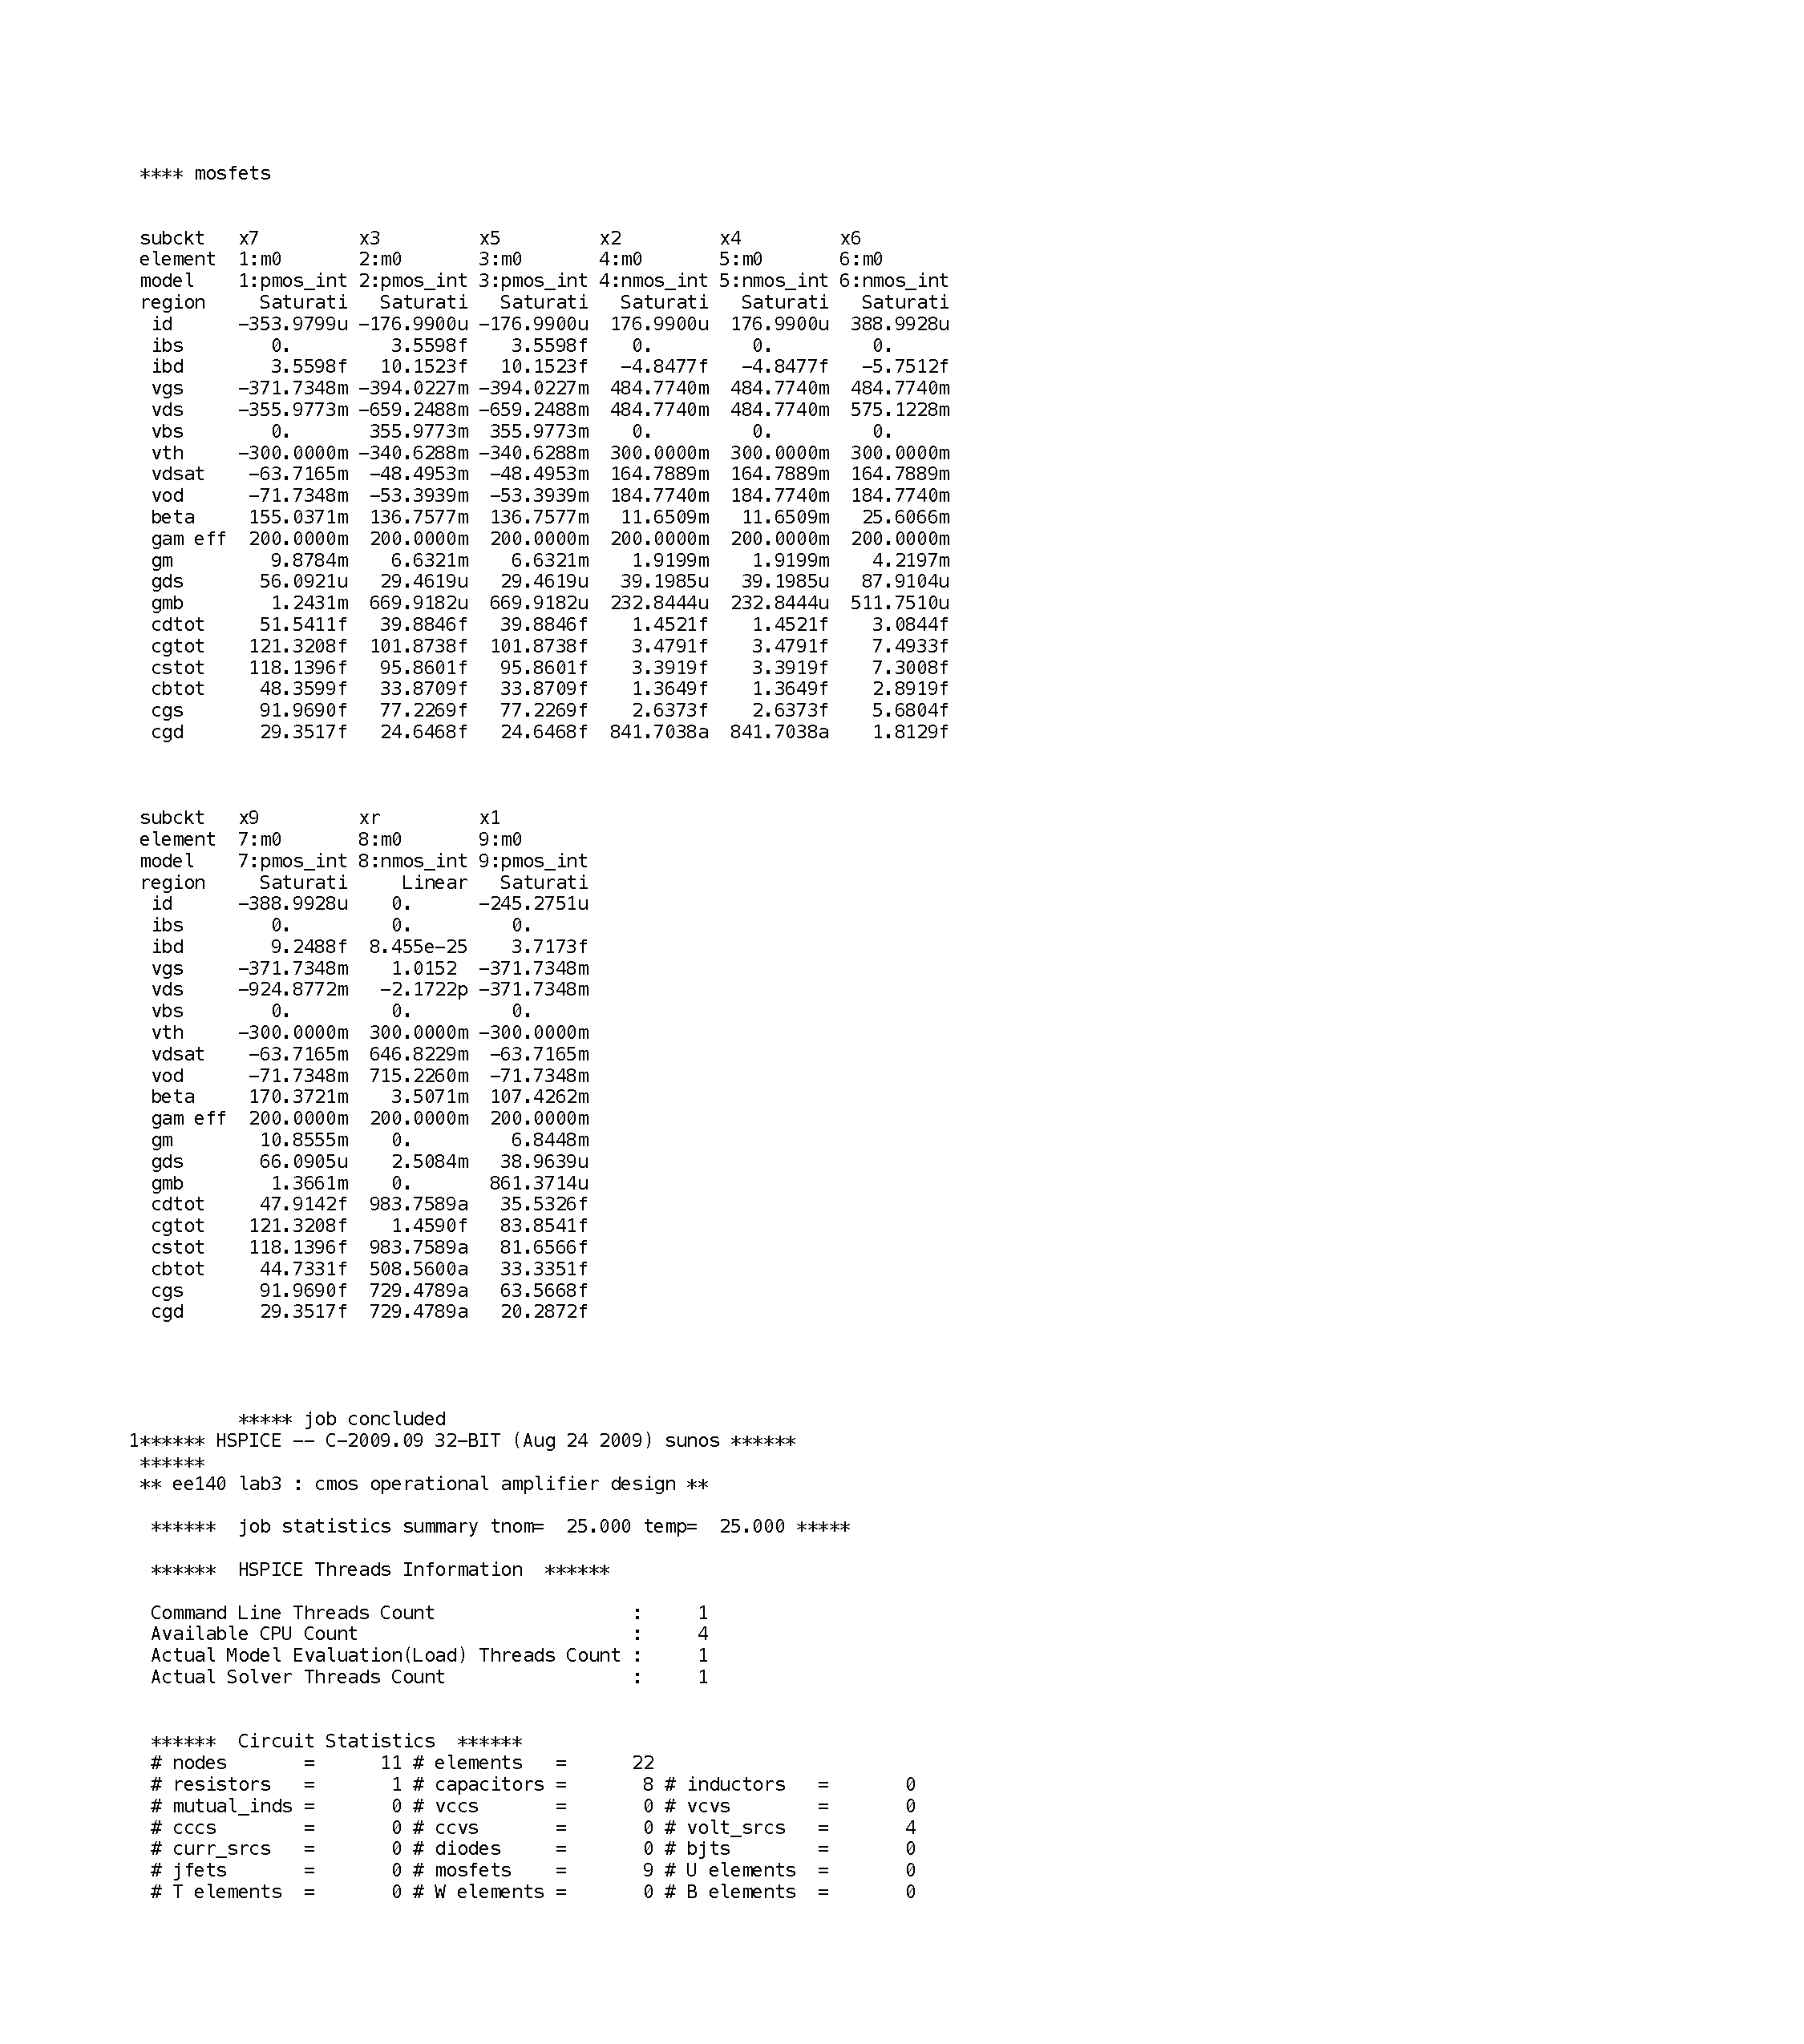
\includegraphics[width=1.3\textwidth]{operating_point_page2.pdf}
			\caption{Summary of biasing and small signal parameters simulated in hspice}
		\end{figure}
		\newpage
		\begin{center}
			\begin{figure}
				\subsubsection{Transistor Dimensions}
				All transistor sizes are within $10\%$ of the expected values from the hand calculations with the exception of $M2,4,6$ and $MR$. $M6$ was manually resized to secure saturation conditions across all transistors. The simulation shows that this transistor is in the linear region when the size is in the range of the hand calculated value. The size of $M6$ was reduced until the transistor was saturated and the output voltage was biased at a value close to $0.75V$. A similar procedure was initially taken with $M2,4$. $MR$ was manually resized to provide a good phase margin. We are able to manually resize this device by pulling the newly simulated value of $gm_{II}$ and adjusting the width until the resistance is approximately equal to $1/gm_{II}$.The result is a circuit that matches all other expected values to within $10\%$ or better.
				$$$$
				
  				\begin{tabular}{ | l | l | l | p{5cm} |}
   			 		\hline
   			 		Transistor & Width & Length &------------\\ \hline
   			 		M1 & 61,100nm & 130nm & \\ \hline
    					M2 & 2,535nm & 130nm & \\ \hline
    					M4 & 2,535nm & 130nm & \\ \hline
					M3 & 74,230nm & 130nm & \\ \hline
					M5 & 74,230nm & 130nm & \\ \hline
					M6 & 5,460nm & 130nm & \\ \hline
					M7 & 88,400nm & 130nm & \\ \hline
					M9 & 88,400nm & 130nm & \\ \hline
					MR & 845nm & 130nm & \\ \hline				
	  			  	\end{tabular}
			\caption{Table of device dimensions.}
			\end{figure}
			\end{center}
			\newpage
			
			\begin{center}
			\begin{figure}
				\subsection{Performance Summary}
  				\begin{tabular}{ | l | l | l | p{2cm} |}
   			 		\hline
   			 		Parameter & Specification & Circuit Performance & Spec Met? \\ \hline
   			 		DC Gain & 1500 & 5121 & Yes\\ \hline
    					Common Mode Input Range & 0.8V & 1.35V & Yes\\ \hline
    					Output Swing & 1.2V & 1.275V & Yes\\ \hline
					Power Dissipation & 1.5mW & 1.48mW & Yes\\ \hline
					Unity Gain Frequency & 600 MHz & 725 MHz & Yes\\ \hline
					Settling Time & 8ns & 7.8ns rising, 7.78ns falling & Yes\\ \hline
					CMRR & 75dB & 83.2dB & Yes\\ \hline
					PSRR at DC & 60dB & 92dB & Yes\\ \hline
					PSRR at 1MHz & 50dB & 94.7dB & Yes\\ \hline
					Lmin & 130nm & 130nm & Yes\\ \hline
					Wmin & 195nm & 845nm & Yes\\ \hline
					Temperature & 25C & 25C & Yes\\ \hline
  			  	\end{tabular}
			\caption{Table of simulated specifications}
			\end{figure}
			\end{center}
			
		\newpage
		
		
		\begin{figure}
			\subsection{DC Gain, Phase Margin, and Unity Gain Frequency}
			The graphs below show the simulated results of the amplifier's open loop gain, frequency response, and phase margin at unity gain.
				\subsubsection{DC Gain}
				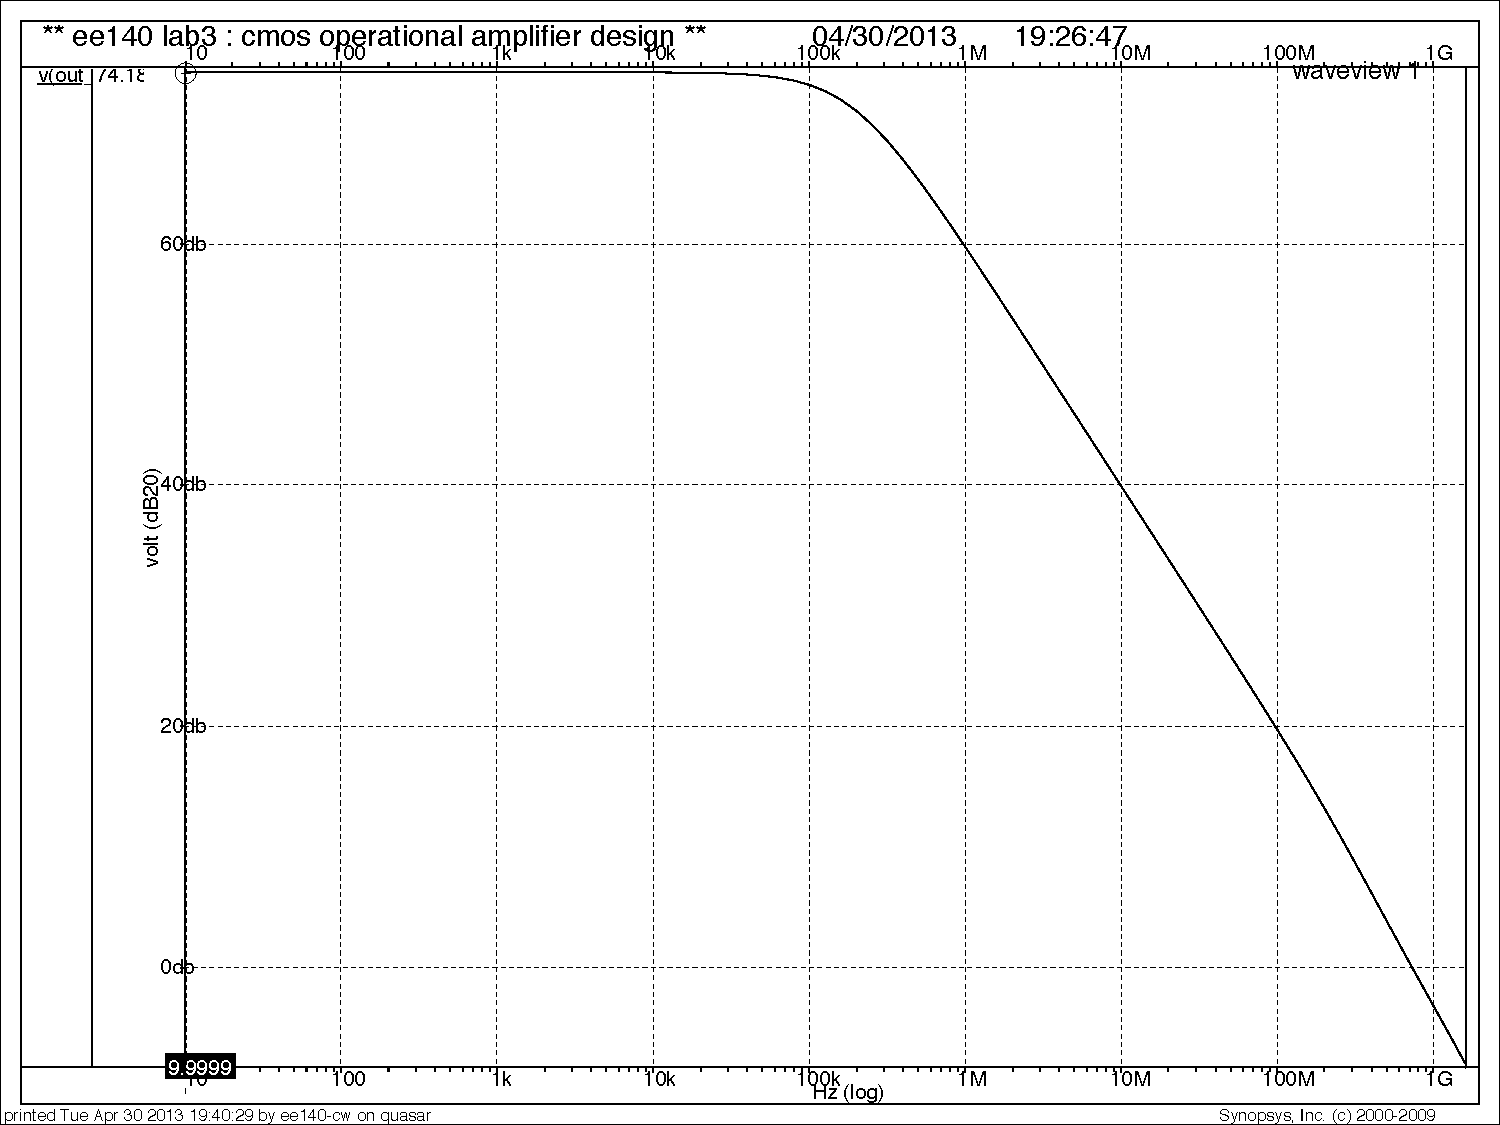
\includegraphics[width=1.1\textwidth]{diff_gain_DC.pdf}
				\caption{The differential gain of the amplifier is $74.18dB$}
		\end{figure}
		
		\begin{figure}
			\subsubsection{ Unity Gain Frequency}
			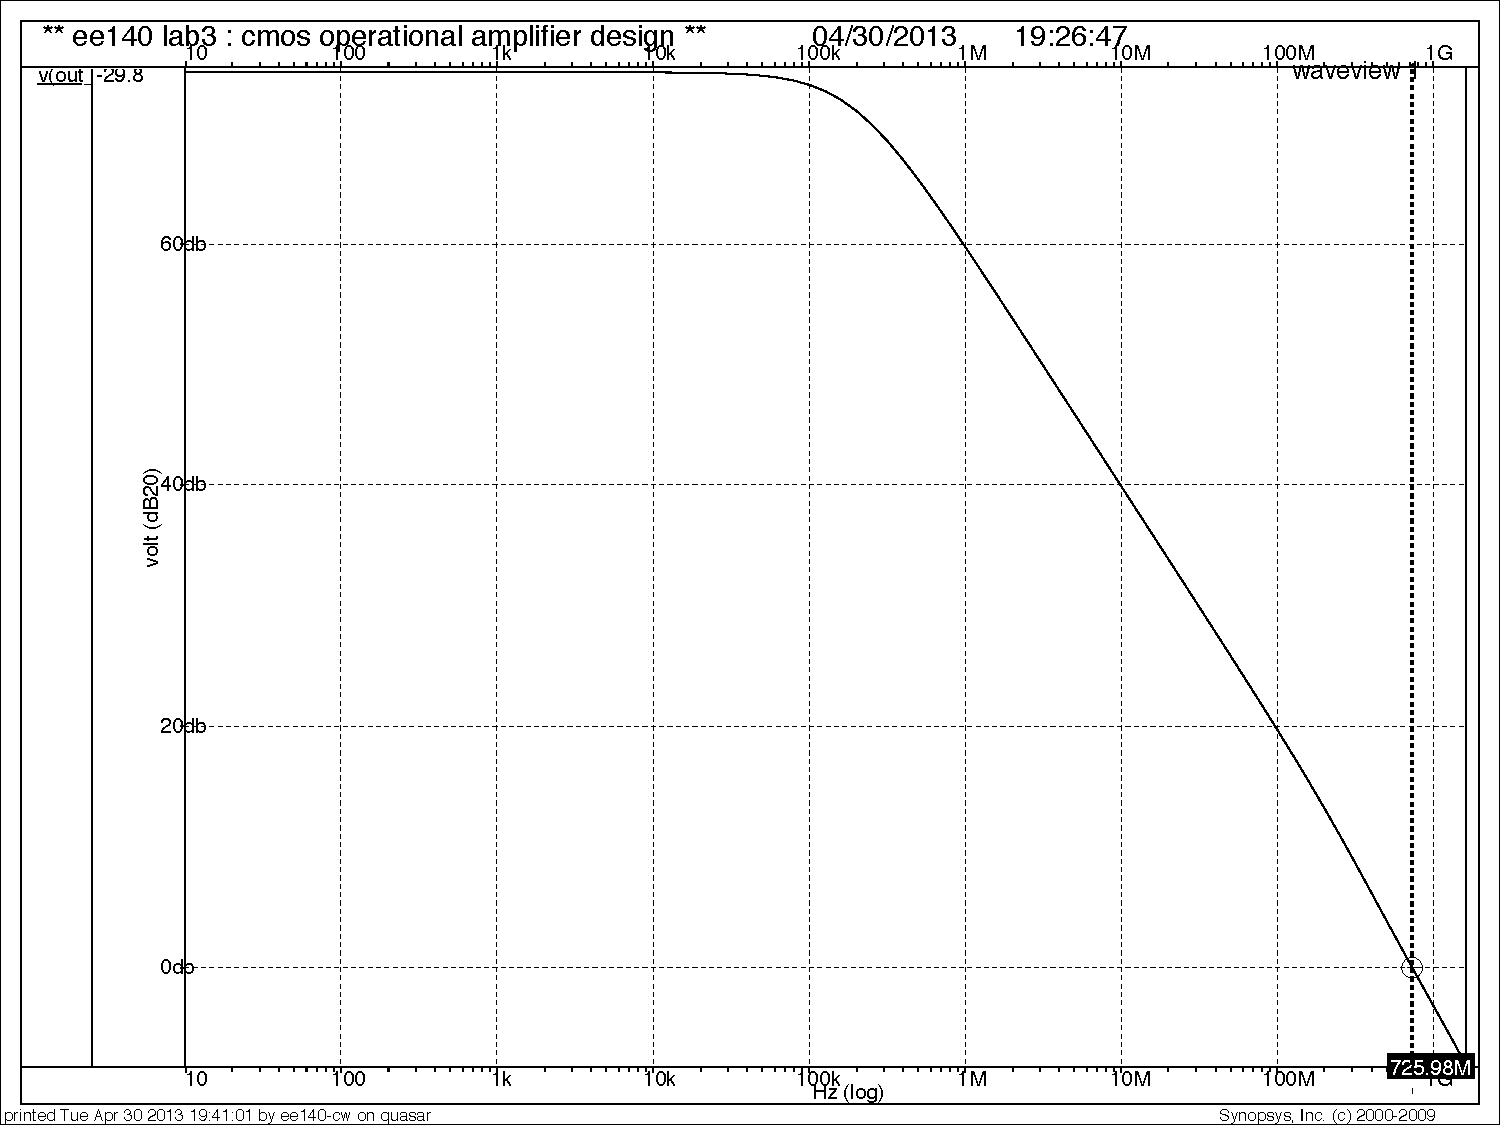
\includegraphics[width=0.9\textwidth]{diff_gain_UNITY.pdf}
			\caption{The unity gain frequency of the amplifier is $725.98MHz$}
			\subsubsection{Phase}
			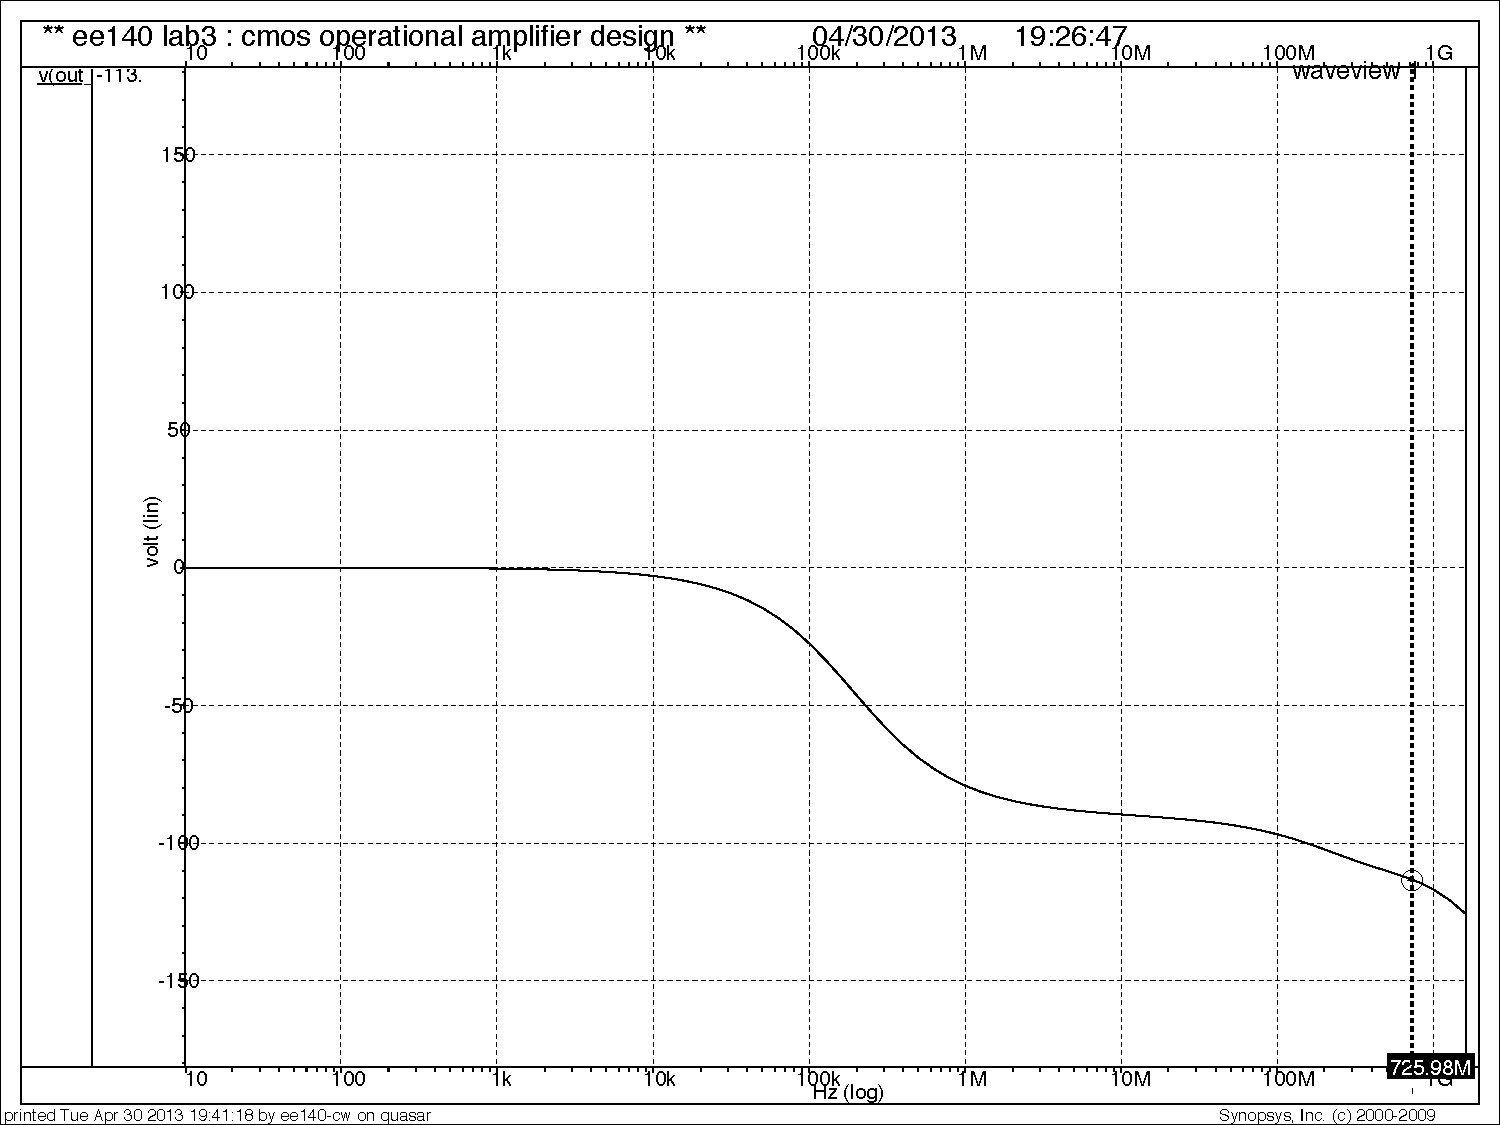
\includegraphics[width=0.9\textwidth]{diff_gain_PHASE.pdf}
			\caption{The phase at unity gain is $-113^{o}$. The phase margin at unity is $67^{o}$}
		\end{figure}
		
		\begin{figure}
			\subsection{CMRR and PSRR}
			The graph below shows the amplifier's common mode rejection ratio and power supply rejection ratio. By taking the ratio of the common mode gain to the differential mode gain, we compute the common mode rejection ratio. By taking the ratio of the power supply gain to the differential mode gain, we compute the power supply rejection ratio. These values can be found in figure 3 above.\\
			\\
			Note that the power supply gain from the negative source can be computed by the equation offered in section 2.1.7. With the amplifier providing a gain on the order of $74$dB at low frequencies and roughly $60$dB at $1MHz$, it is clear that $PSRR_{-} > 60dB$.
				\subsubsection{Common mode gain}
				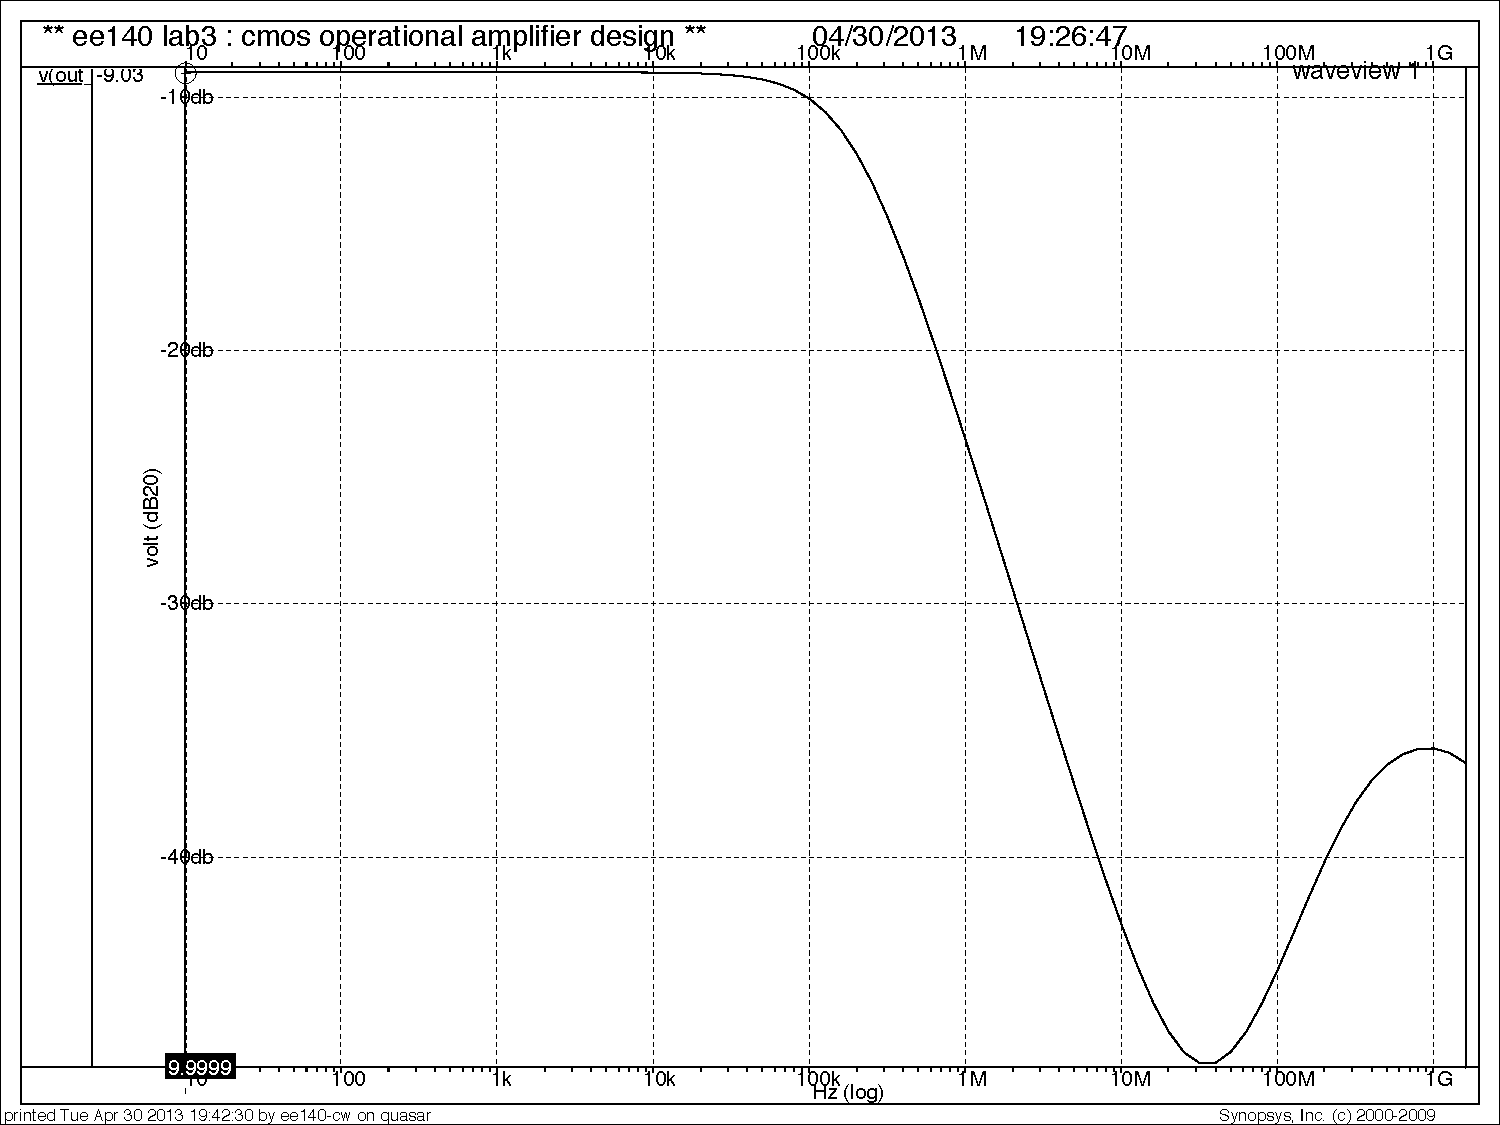
\includegraphics[width=1.1\textwidth]{cmrr_DC.pdf}
				\caption{The common mode gain of the amplifier is $-9.03dB$}
		\end{figure}
		
		\begin{figure}
			\subsubsection{ Power supply gain at DC}
			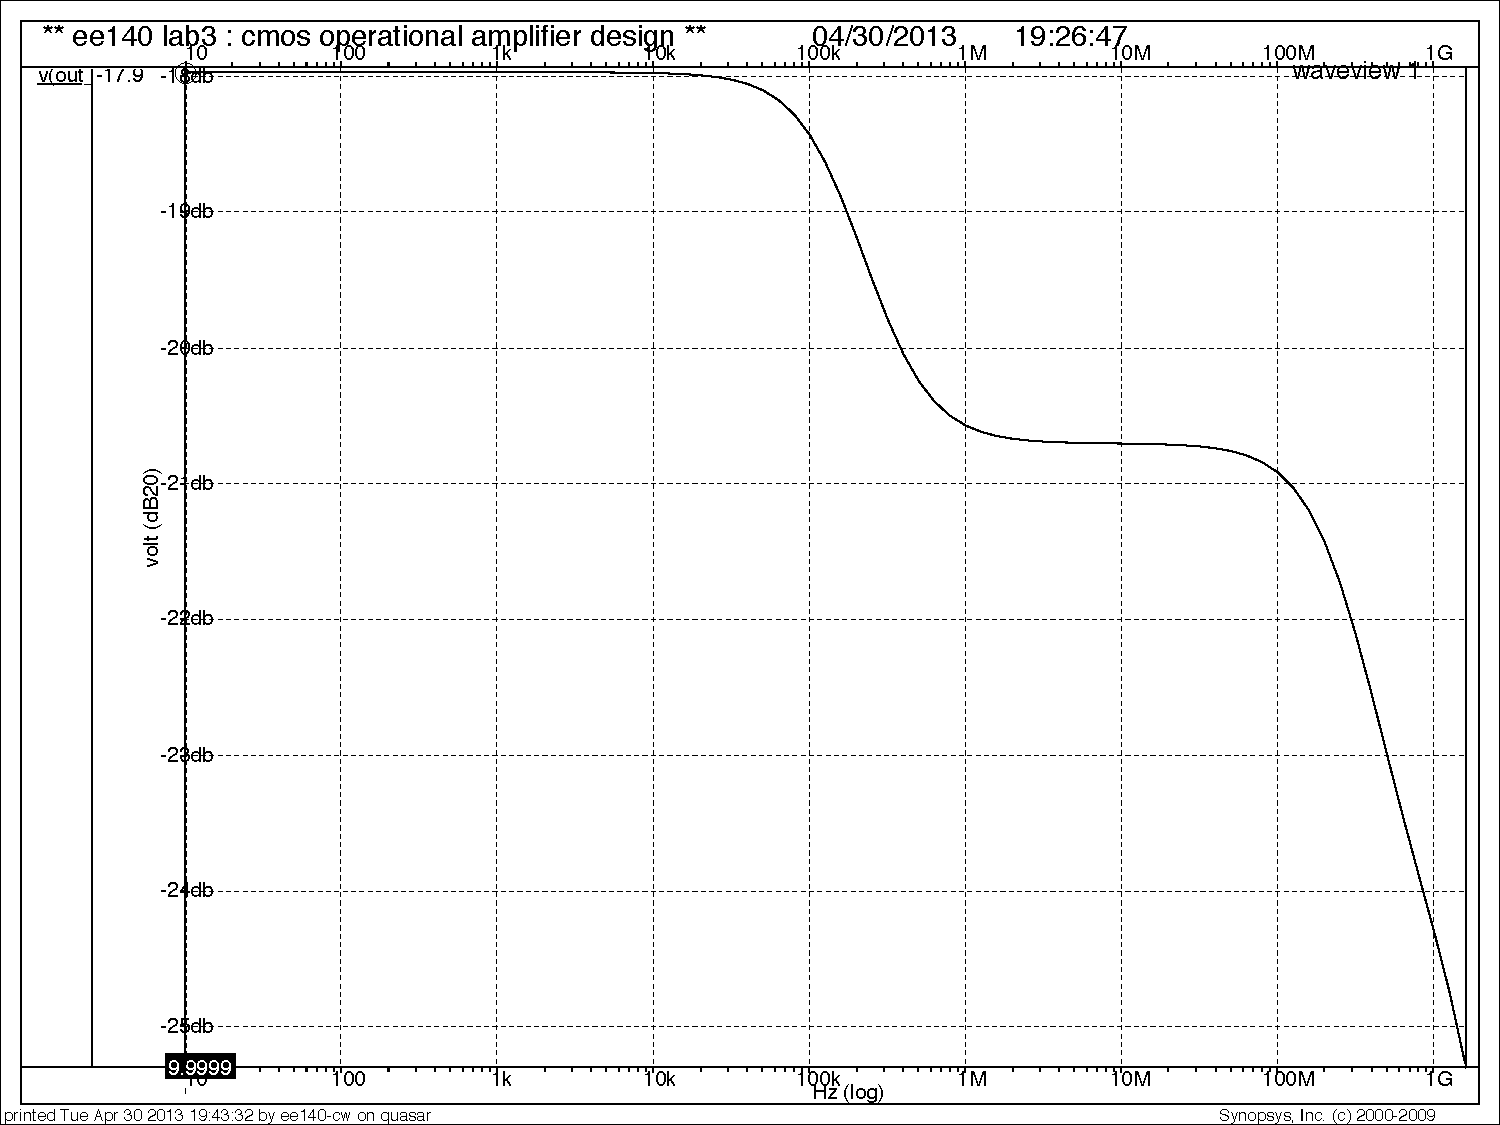
\includegraphics[width=0.89\textwidth]{psrr_DC.pdf}
			\caption{The power supply gain at $DC$ is $-17.9dB$}
			\subsubsection{Power supply gain at 1MHz}
			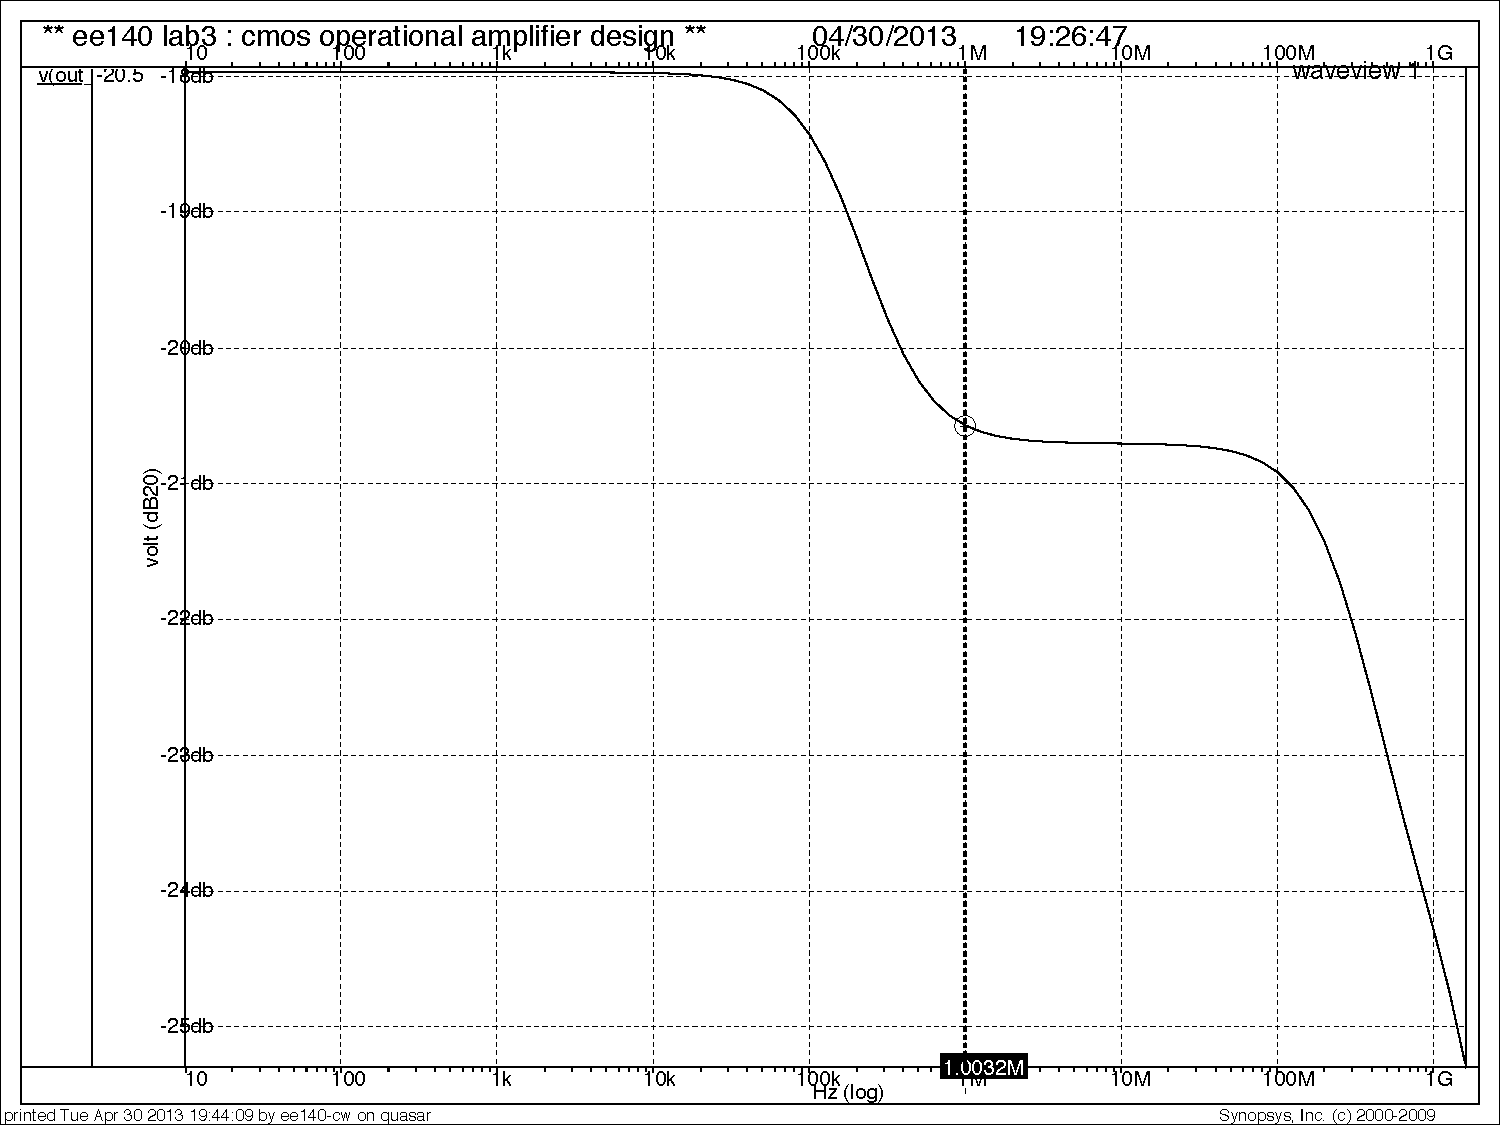
\includegraphics[width=0.89\textwidth]{psrr_1MHz.pdf}
			\caption{The power supply gain at $1MHz$ is $-20.5dB$}
		\end{figure}
		
		\begin{figure}
			\subsection{Common Mode Input Range}
			This is defined as the range of voltages at which $dVout/dVin$ becomes $1/2$ in unity gain feedback. To show this, we put the op amp into unity gain configuration and sweep the $DC$ voltage at the input from 0 to $V_{DD}$. The graphs below show the maximum and minimum of this range. This amplifier exceeds the specification by a relatively large margin. This is partly due to tying the bulk to $V_{DD}$ in $M3,5$. This was done because the body effect on the input transistors can be used to increase the range\footnote{\tiny Paul Gray, Robert Meyer, "Analysis and Design of Analog Integrated Circuits" (Wiley and Sons, 2010), 428}. The total common mode input range of the amplifier is listed in figure 3.
				\subsubsection{Common Mode Input Range, minimum}
				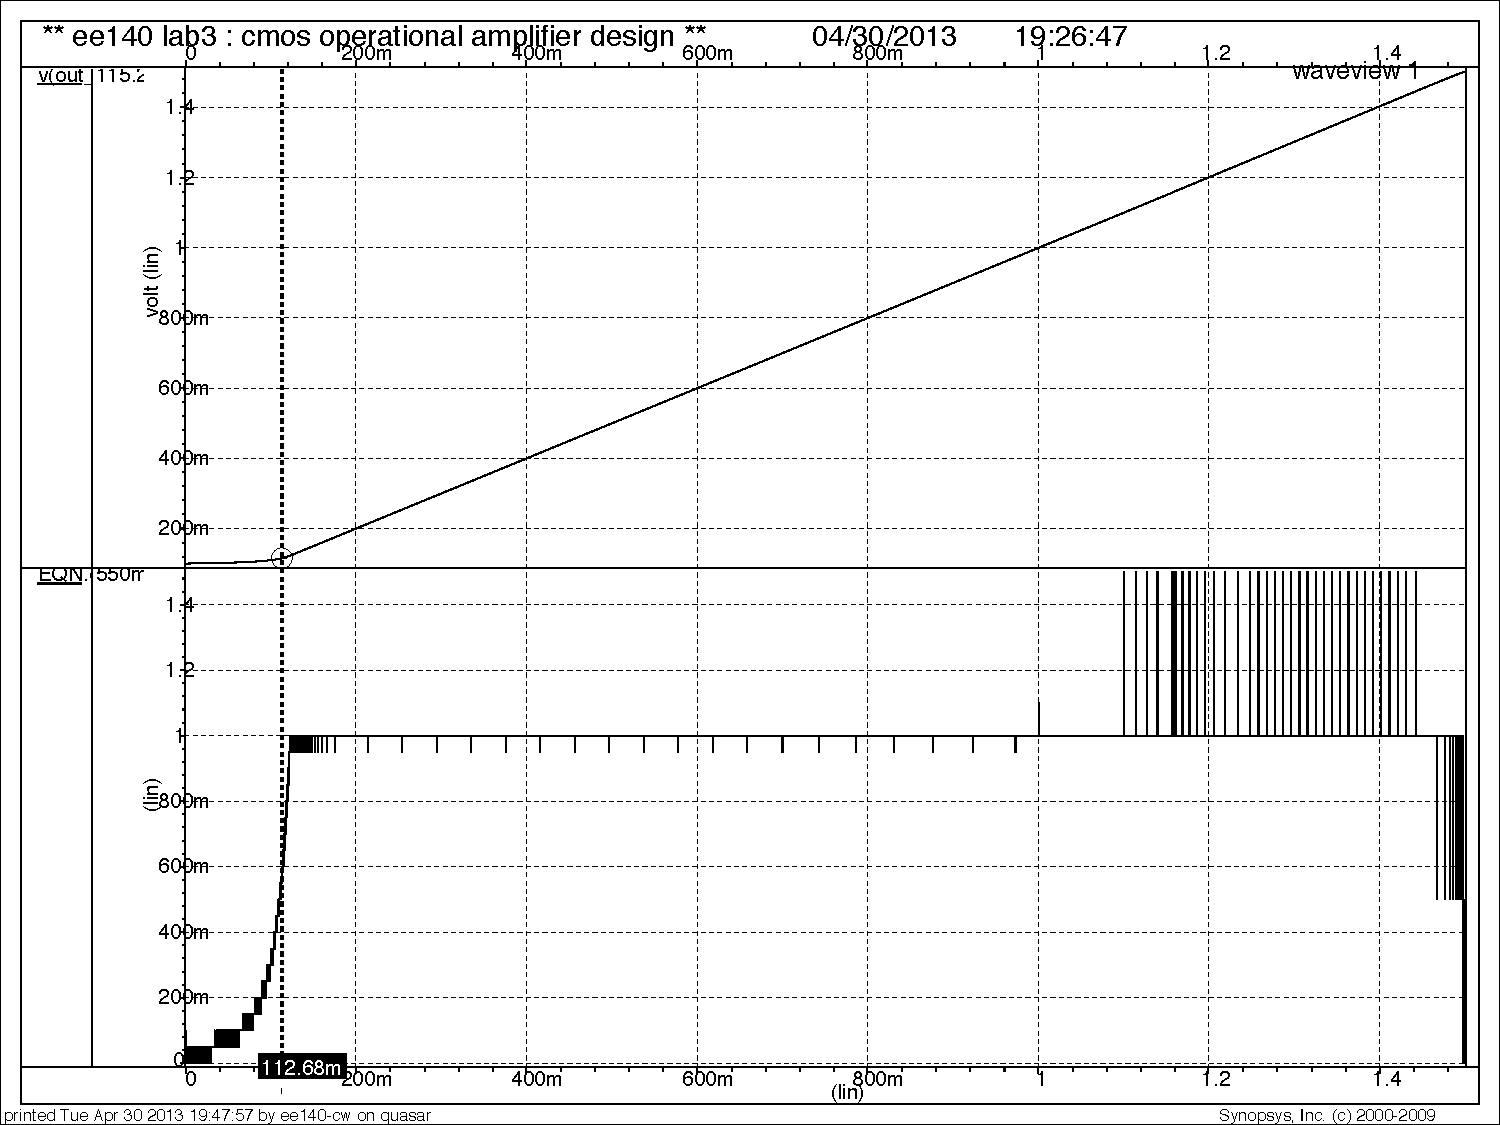
\includegraphics[width=0.6\textwidth]{common_mode_input_range_1.pdf}
				\caption{The minimum value corresponds to an output voltage of $0.115V$}
				\subsubsection{Common Mode Input Range, maximum}
				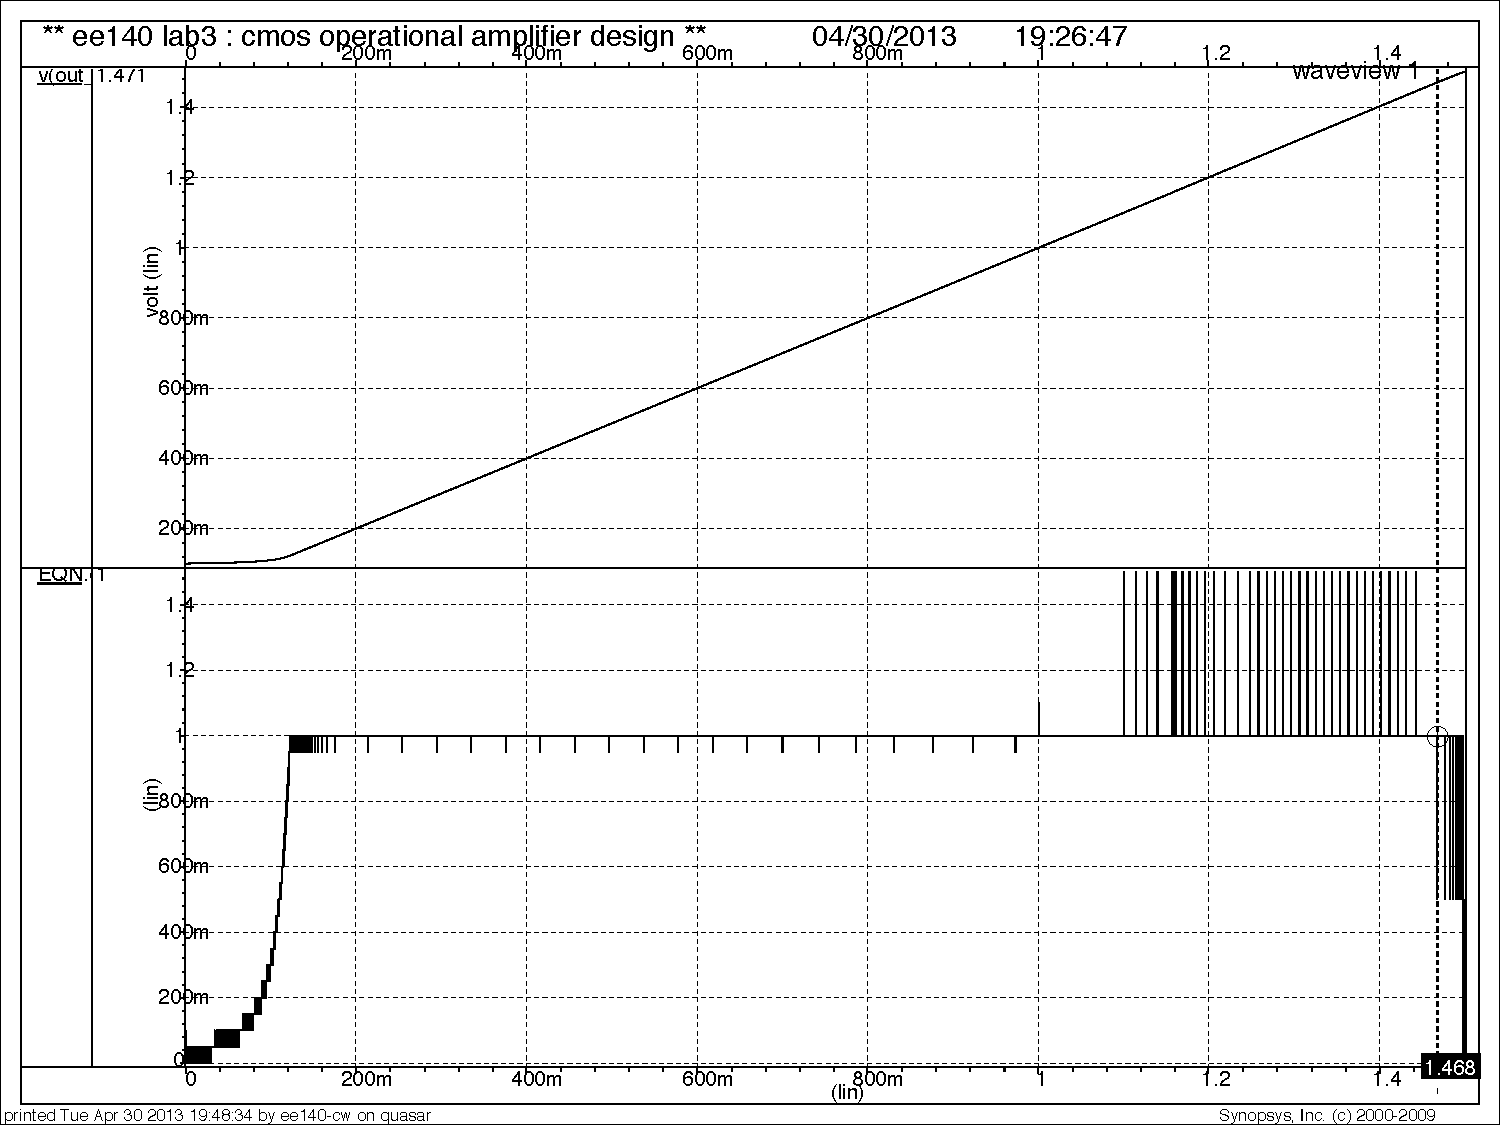
\includegraphics[width=0.6\textwidth]{common_mode_input_range_2.pdf}
				\caption{The maximum value corresponds to an output voltage of $1.47V$}

		\end{figure}
		
		\begin{figure}
			\subsection{Output Swing}
			This is defined as the range of voltages at which $dVout/dVin$ becomes $1/10th$ the nominal differential gain. To show this, we sweep the $DC$ voltage at one of the inputs around its bias points and find the points on the curve where the derivative is approximately equal to $1/10th$ of the nominal gain. The graphs below show the minimum and maximum of this range. The total output swing of the amplifier is listed in figure 3.
				\subsubsection{Output Swing, minimum}
				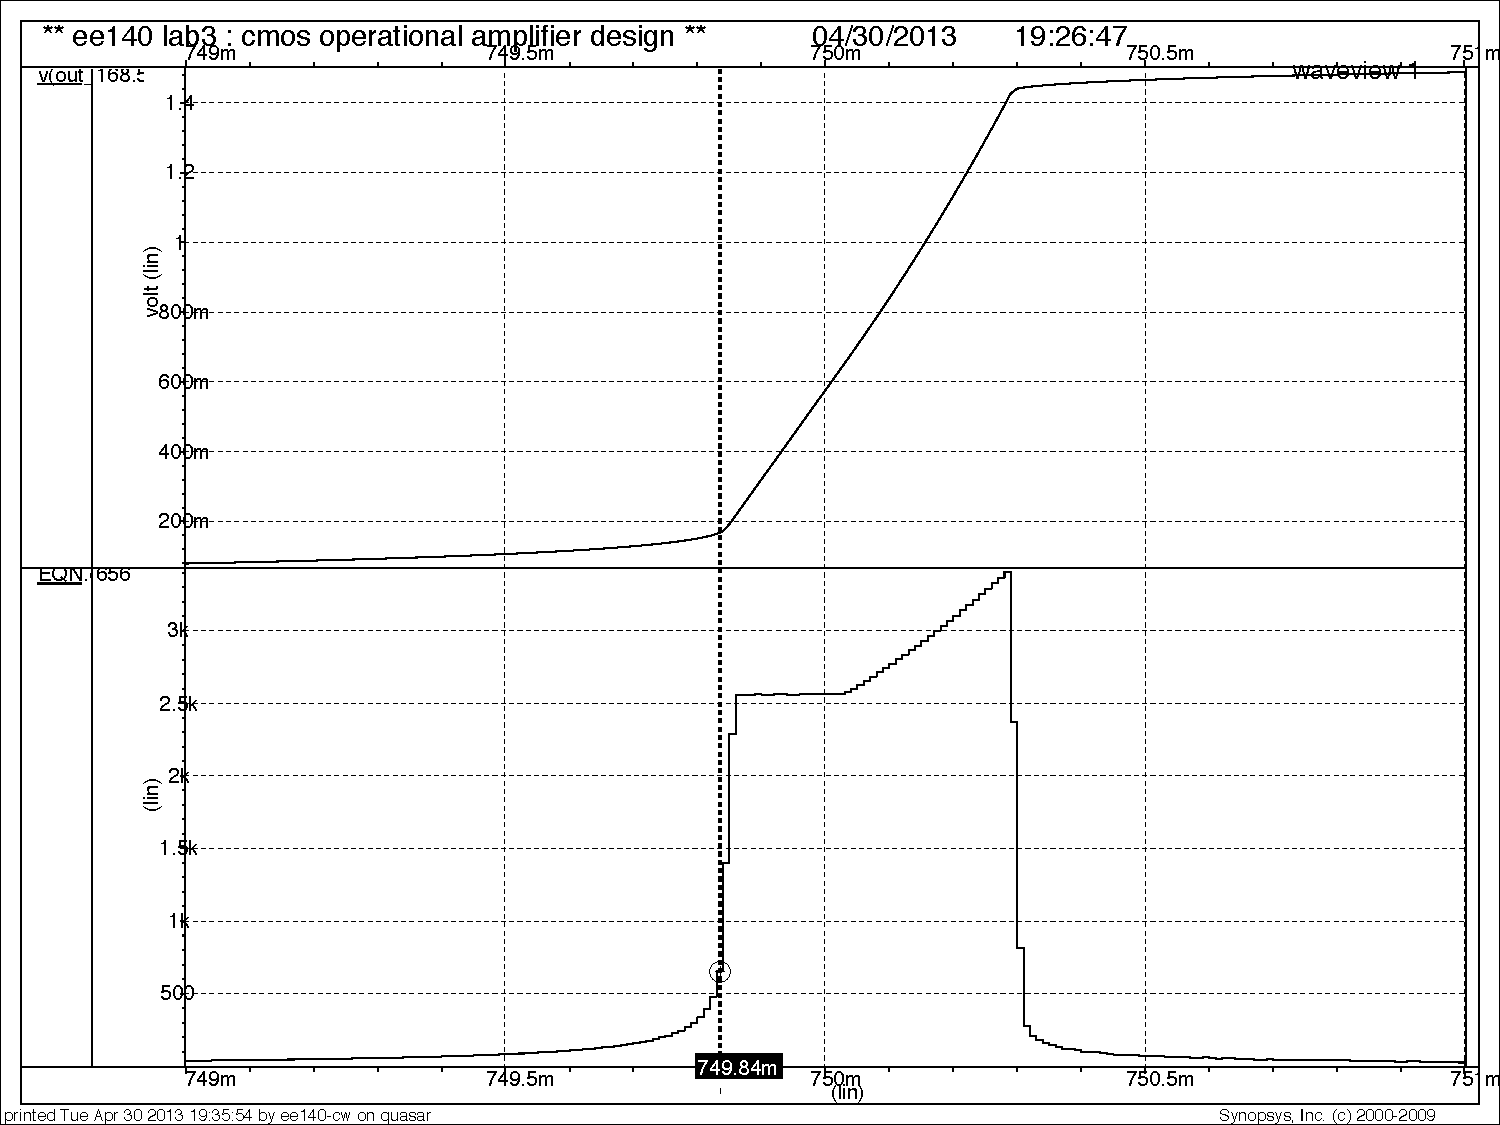
\includegraphics[width=0.65\textwidth]{output_swing.pdf}
				\caption{The minimum value corresponds to an output voltage of $0.168V$}
				\subsubsection{Output Swing, maximum}
				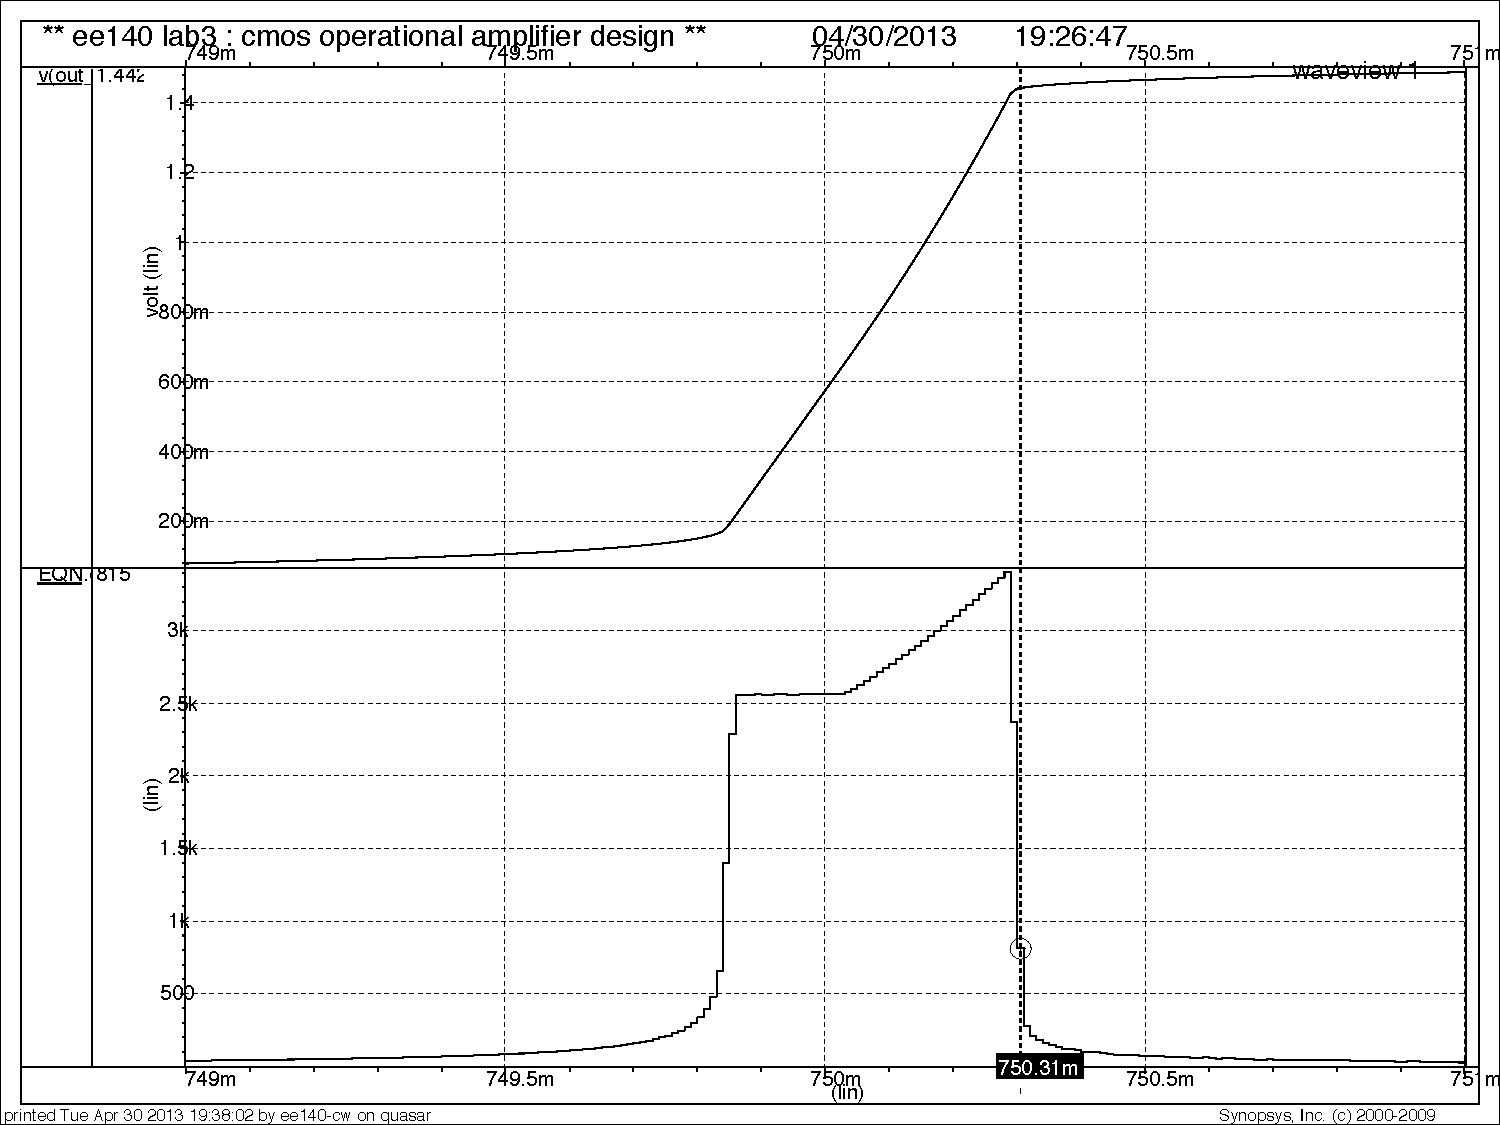
\includegraphics[width=0.65\textwidth]{output_swing_2.pdf}
				\caption{The maximum value corresponds to an output voltage of $1.44V$}

		\end{figure}
		
		\begin{figure}
			\subsection{Settling Time}
			This is the most stringent specification to meet, as it requires relatively large amounts of current to be supplied from the current sources. We measure settling time by putting the op amp into unity gain feedback and applying a $0.4V$ step to the input. We then run a transient analysis in hspice to determine the time it takes for the amplifier's output to converge to within $0.1\%$. The time it takes to converge must be under $8$ns.\\ \\
			In order to meet this specification, some changes to device dimensions were made in order to increase the current to a value high enough to just meet the spec. Increasing the sizes of the current sources allowed for a better settling time; the drawback however, is that power consumption became excessive. To ameliorate this, the size of the biasing transistor was reduced and the bias resistor increased in order to preserve roughly the same overdrive voltage. The result is an amplifier that has a settling time of just under $8$ns and consumes less than $1.5$mW of power.
				\subsubsection{Settling Time}
				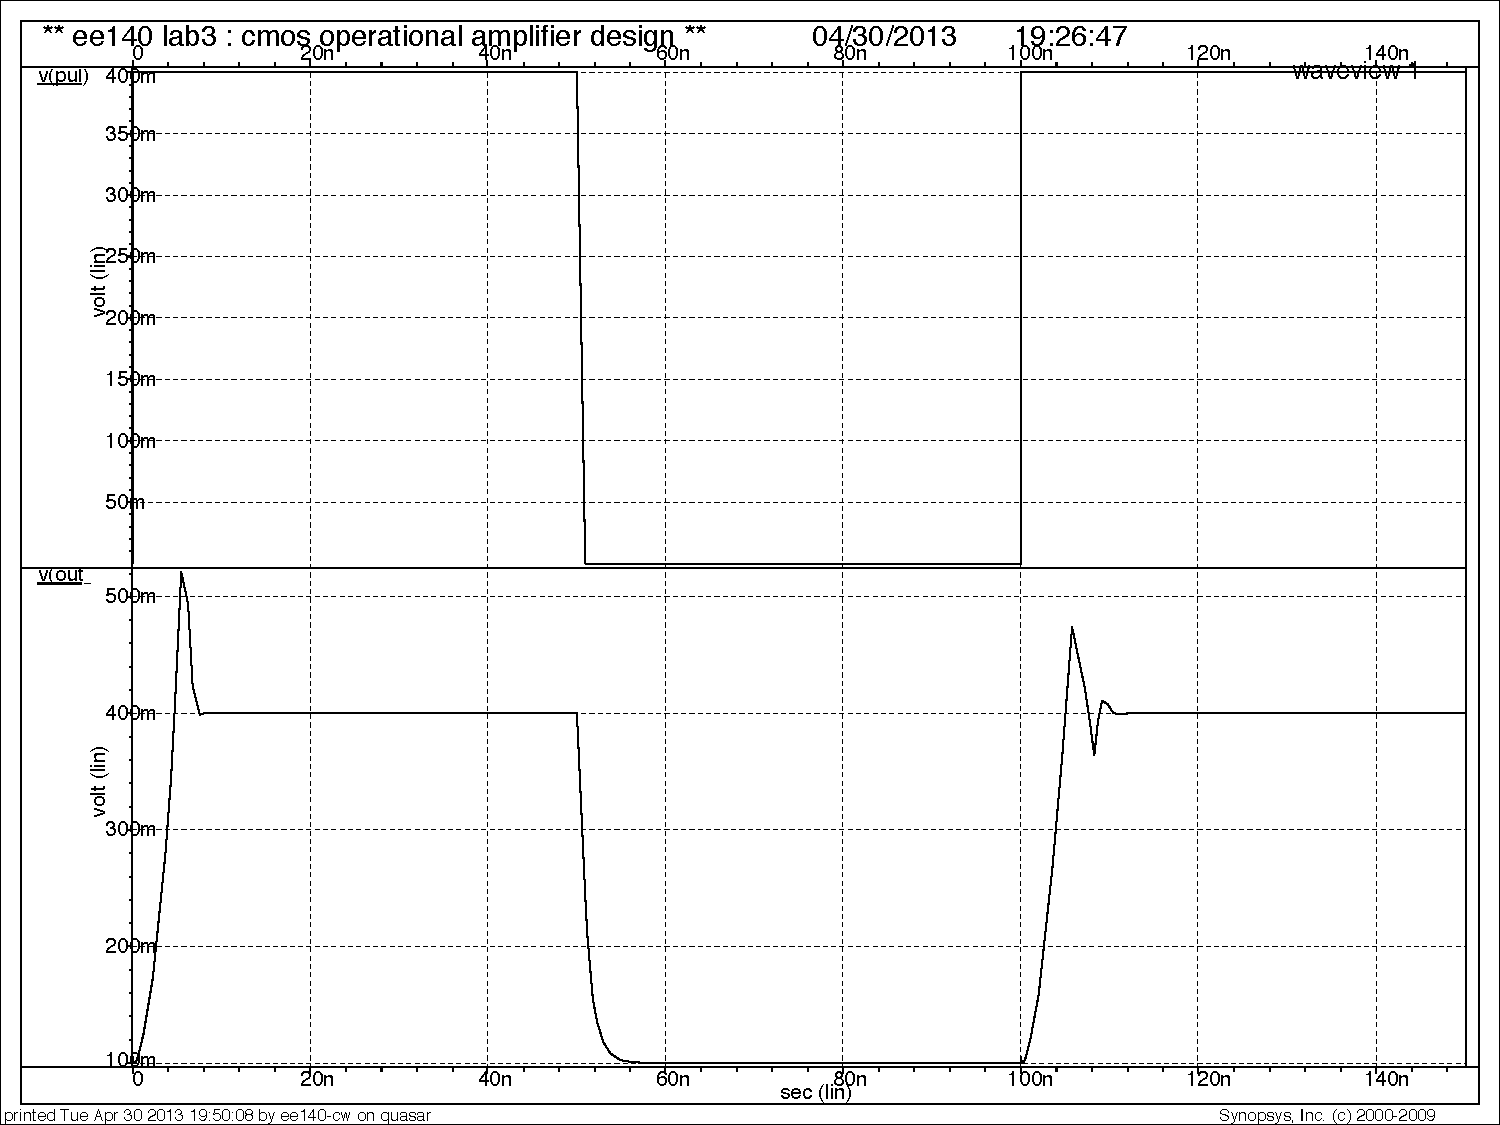
\includegraphics[width=1.1\textwidth]{settling_time_zoomed_out.pdf}
				\caption{$0.4V$ step input and amplifier response}
		\end{figure}
		
		\begin{figure}
				\subsubsection{Settling Time, rising input}
				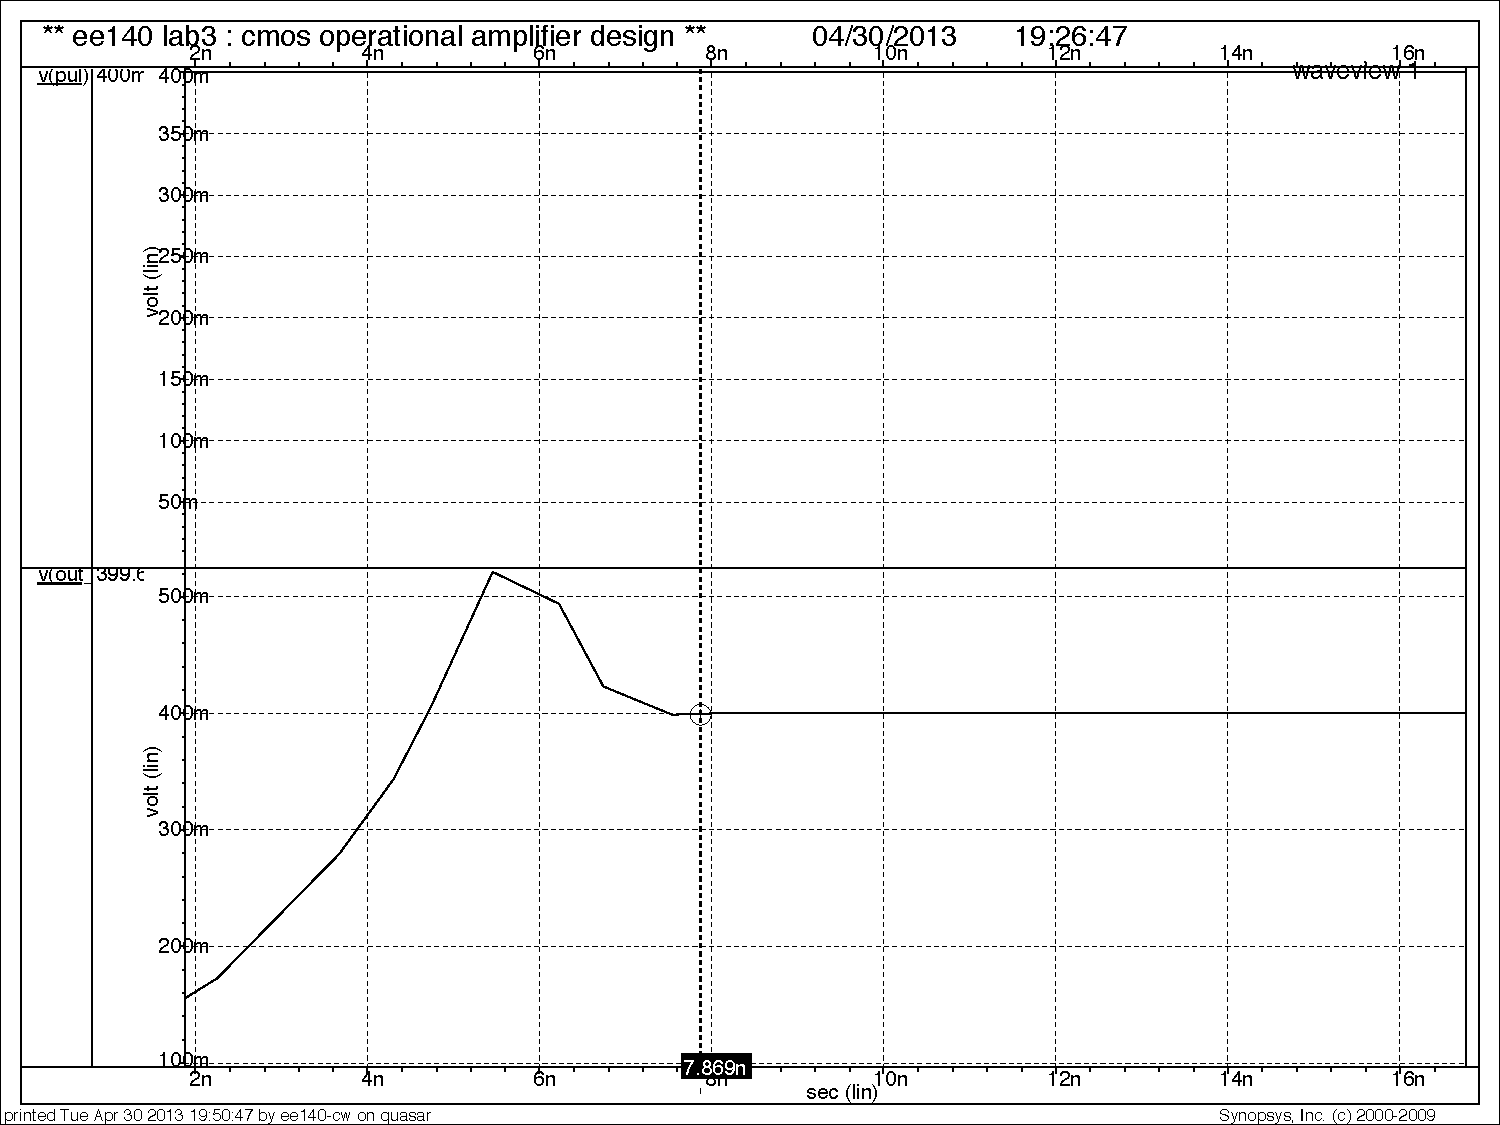
\includegraphics[width=0.8\textwidth]{settling_time_t1.pdf}
				\caption{The time it takes to converge on a rising input is $7.88ns$}
		\end{figure}
		
		\begin{figure}
				\subsubsection{Settling Time, falling input}
				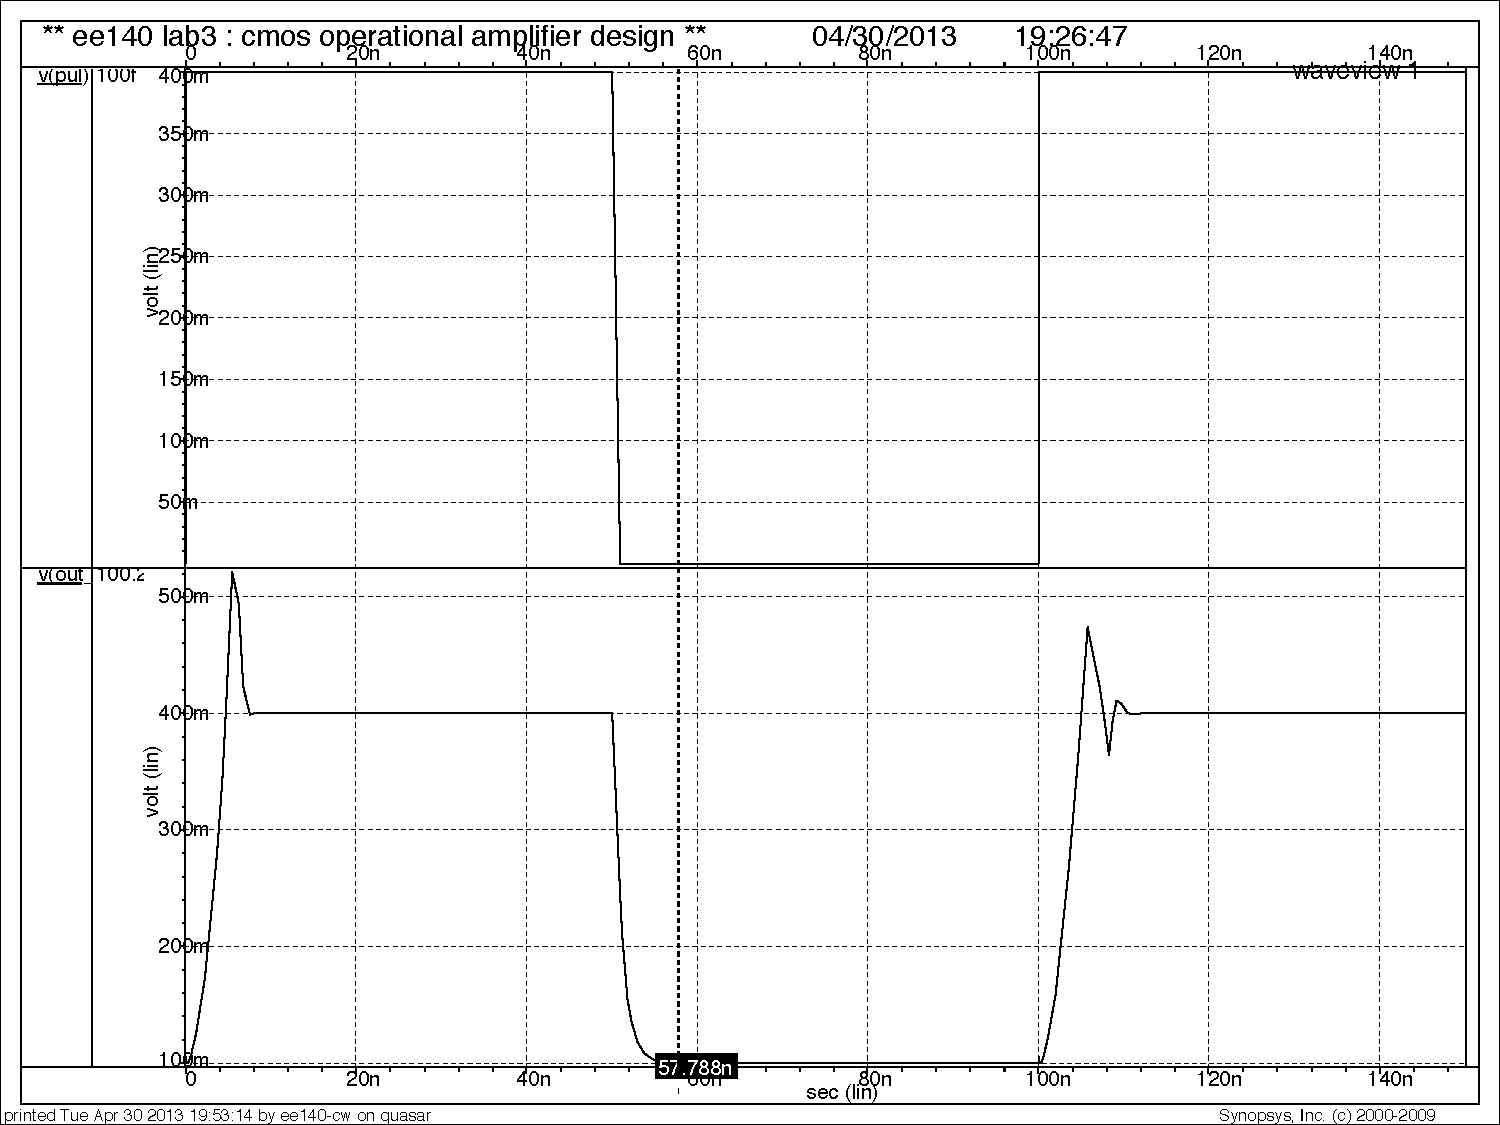
\includegraphics[width=0.8\textwidth]{settling_time_t2.pdf}
				\caption{The time it takes to converge on a falling input is $7.78ns$}
		\end{figure}
		\pagebreak
		...
		\newpage
		\section{Conclusion}
			We have shown the design process of an analog integrated circuit CMOS operational amplifier, and we have shown how equations we have derived throughout the semester participate in this process. We have seen how tradeoffs must be made between certain parameters in order to provide an amplifier that is balanced and meets a wide range of specifications. For the most part, the amplifier considered in this paper is ideal for use in digital circuits or mixed signal circuits where the characteristics of the stages connected to the op-amp are known in advance. This amplifier provides a good gain for digital signals (digital signals typically do not require as much gain as their analog counterparts), a wide bandwidth, stellar phase margin for gains down to and below unity, a very quick settling time, and consumes very little power. Furthermore, the amplifier has a very good power supply rejection ratio which offers outstanding performance in digital circuits with high levels of switching noise. Overall, the amplifier we have designed is a stable, low power op-amp that is the quintessential CMOS operational amplifier utilized by engineers throughout the world.
			$$$$
			The design of this op amp was a scrupulous and testing process, and a tremendous learning experience as well. To see how all of the many variables depended on each other required me to think in a way that I have never before and forced me to stretch and expand my mind to such great heights. Arguably, a better way to design a circuit like this is to write a geometric program and have a computer automatically compute a robust design given the parameters and specifications. This implies that the circuit designer can spend more time doing real design, $i.e.,$ carefully analyzing the optimal trade-offs between competing objectives and less time doing parameter tuning or wondering whether a certain set of specifications can be achieved. However, for the purposes of this course and the learning experience required to become a competent circuit designer, it is necessary to do this type of analysis by hand and think about the circuit ourselves, rather than have a computer do the thinking for us. At the end of the day, I can say that I have a solid grasp and comprehension of the way a relatively large MOS circuit like this operates. I realize the interdependencies between variables like dimension, transconductance, and overdrive voltage, and I acknowledge the tradeoffs required to satisfactorily meet an extensive range of specifications. Overall, the wisdom and erudition bestowed upon me as a result of successfully completing this project is immense, and it was undeniably worth the effort.
		
	
	
\end{document}